\apendice{Especificación de diseño}

\section{Introducción}

A continuación se presentan los diseños elaborados para poder realizar los objetivos anteriores. Se ha incluido el diagrama de despliegue, el diseño de datos, el diseño procedimental y el diseño arquitectónico.

\section{Diagrama de despliegue}

Como se puede ver reflejado en la figura~\ref{img:diagramaDespliegue}, la aplicación cuenta con 3 bloques claramente diferenciados:

\begin{itemize}
	\item El navegador personal del cliente donde se ejecuta la aplicación. 
	\item Un servidor web con \textit{Apache} instalado en el que se despliega un proyecto en \textit{CakePHP}.
	\item Un servidor de base de datos donde se aloja una base de datos relacional de \textit{MySQL}.
\end{itemize}

\begin{figure}[h]
	\centering
	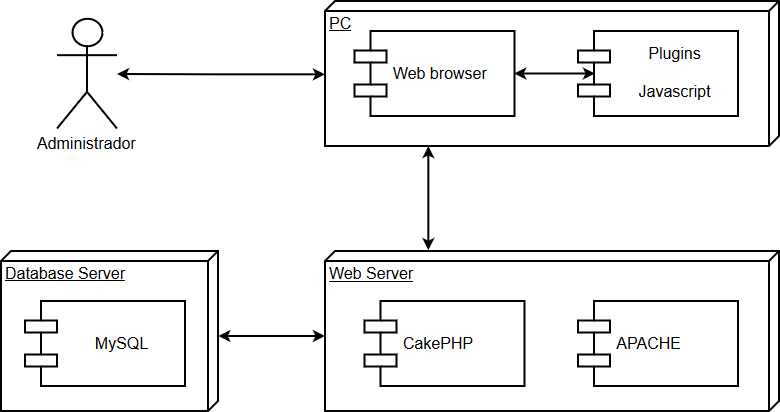
\includegraphics[width=1\textwidth]{/anexos/Diseno/DiagramaDespliegue}
	\caption{Diagrama de despliegue de la aplicación.}
	\label{img:diagramaDespliegue}
\end{figure}

\section{Diseño de datos}

La estructura de datos presentada en este proyecto se recoge en una base de datos relacional \textit{MySQL}. En un primer momento se construyó el diagrama entidad relación a través del cual se obtuvo el diagrama relacional. Durante el proceso de diseño del diagrama entidad relación, se construyó una segunda versión para hacer más fácil su comprensión. En las figuras~\ref{img:modeloER}, ~\ref{img:modeloER2} y~\ref{img:modeloRelacional} se presentan las dos versiones de los modelos entidad relación y relacional respectivamente.

Antes de continuar, se considera oportuno hacer algún apunte acerca de ambos diagramas.

En el diagrama entidad-relación, se puede destacar como elemento llamativo la relación \textit{ISA}. Dado que una tecnología no puede ser renovable y fósil a la vez y no hay una tecnología que no sea renovable ni fósil, se va a clasificar esta \textit{ISA} como exclusiva total. 
Otro punto a tener en cuenta es cómo se ha resuelto la relación ternaria, ya que se ha creado la tabla \textit{rangerenewables} para simplificar y unificar la relación.

En cuanto a las entidades débiles, el discriminante se representa con lineas discontinuas. Ya para todas las tablas, al modelar un diagrama entidad relación, prescindimos de representar las claves ajenas, si presentes en el diagrama relacional.

A continuación se recogerá en un diccionario de datos cada una de las tablas generadas con sus correspondientes campos y las unidades si son relevantes:

\begin{itemize}
	
	\item \textit{countries}: Los países presentes en la instalación.
	\begin{itemize}
		\item \textit{id}: Identificador del país.		
		\item \textit{name}: Nombre del país.
	\end{itemize}
	
	\item \textit{regions}: Cada una de las regiones pertenecientes a un país.
	\begin{itemize}
		\item \textit{id}: Identificador de la región.		
		\item \textit{id\_country}: Identificador del country al que pertenece.
		\item \textit{name}: Nombre de la región.
		\item \textit{dem\_for}: Margen de reserva por error en el pronostico de demanda.
		\item \textit{ren\_for}: Margen de reserva por error en el pronostico de generación renovable.
	\end{itemize}

	\item \textit{arcs}: Comunicación entre dos regiones.
	\begin{itemize}
		\item \textit{id}: Identificador del arco.		
		\item \textit{id\_region\_1}: Identificador de la región de origen.
		\item \textit{id\_region\_2}: Identificador de la región de destino.
		\item \textit{distance}: Distancia entre 2 regiones (Km).
	\end{itemize}
	
	\item \textit{fuels}: Tipos de combustibles.
	\begin{itemize}
		\item \textit{id}: Identificador del combustible.		
		\item \textit{name}: Nombre del combustible.
		\item \textit{fue\_cos}: Coste por unidad de combustible importado. (\textdollar/MMBTU).
		\item \textit{production}: Reserva nacional de combustible. (MMBTU).
	\end{itemize}
	
	\item \textit{technologies}: Tipos de tecnologías renovables y no renovables.
	\begin{itemize}
		\item \textit{id}: Identificador de la tecnología.		
		\item \textit{name}: Nombre de la tecnologia.
		\item \textit{renewable}: Si es una tecnología renovable $ ([0 - 1]) $
		\item \textit{wat\_wit}: Desperdicio de agua por generación de un \textit{megawhatt}. $ (m^{3}/MWh) $.
		\item \textit{genco\_pri}: Precio de mercado por \textit{megawhatt} $ (\textdollar/MWh) $.
		\item \textit{cap}: Capacidad de planta $ (MW) $.
		\item \textit{new\_cap\_cos}: Costo por \textit{megawhatt} debido a la instalación. $ (\textdollar/MW) $.
		\item \textit{man\_cos}: Costo por \textit{megawhatt} debido al mantenimiento de plantas viejas $ (\textdollar/MWh) $.
		\item \textit{man\_cos\_new\_cap}: Costo por \textit{megawhatt} debido al mantenimiento de plantas nuevas. $ (\textdollar/MWh) $.
		\item \textit{gen\_cos}: Costo por \textit{megawhatt-hora} generado para plantas viejas. $ (\textdollar/MWh) $.
		\item \textit{gen\_cos\_new\_cap}: Costo por \textit{megawhatt-hora} generado para plantas nuevas. $ (\textdollar/MWh) $.
		\item \textit{life\_time}: Vida util de las plantas de generación.
		\item \textit{ghg\_emi}: Toneladas de $CO_{2}$ producidas por \textit{megawhatt-hora}. $(CO_{2}/MWh)$.
		\item \textit{inv\_cap\_emp}: Empleo en la construcción de las plantas de generación.
		\item \textit{man\_cap\_emp}: Empleo en el mantenimiento de las plantas de generación.
		\item \textit{dec\_cam\_emp}: Empleo en el desmantelamiento de plantas de generación.
		\item \textit{om\_cap\_emp}: Empleo en la operación de plantas de generación.
		\item \textit{fue\_cap\_emp}: Empleo en la producción, procesamiento y transporte de combustibles.
		\item \textit{wat\_con}: Consumo de agua por generación de un \textit{megawhatt} $ (m^{3}/MWh) $.
	\end{itemize}

	\item \textit{typelines}: Tipo de conexión de los arcos entre dos regiones.
	\begin{itemize}
		\item \textit{id}: Identificador del tipo de linea.		
		\item \textit{lin\_cap}: Capacidad de transmisión de linea.
		\item \textit{tension}: Tensión de la linea. $ (MW) $
		\item \textit{new\_lin\_cos}: Costo por kilómetro de instalación. $ (\textdollar/Km) $
		\item \textit{man\_lin\_cos}: Costo por kilómetro de mantenimiento. $ (\textdollar/Km) $
		\item \textit{flo\_cos}: Costo por transmisión de un MWh. $ (\textdollar/MWh) $
		\item \textit{eff\_lin\_bas}: Porcentaje base de eficiencia de la línea (a una temperatura de 20ºC). $ ([0,1]) $
	\end{itemize}

	\item \textit{arcs\_typelines}: Relación entre el arco y el tipo de arco.
	\begin{itemize}
		\item \textit{id\_arc}: Identificador del arco.
		\item \textit{id\_typeline}: Identificador del tipo de linea.
		\item \textit{num\_lines}: Número de lineas de cada tipo.
	\end{itemize}
	
	\item \textit{fuels\_technologies}: Relación entre el combustible y la tecnología.
	\begin{itemize}
		\item \textit{id\_fuel}: Identificador del combustible.
		\item \textit{id\_technology}: Identificador de la tecnología.
		\item \textit{perc\_con}: Porcentaje de aportación de combustibles para generación. $ (0 - 1) $
		\item \textit{fue\_con}: Consumo de combustible necesario para generar un \textit{megawhatt} $ (MMBTU/MWh) $
	\end{itemize}

	\item \textit{regions\_technologies}: Relación entre la región y qué tecnología hay presente.
	\begin{itemize}
		\item \textit{id\_region}: Identificador de la región.
		\item \textit{id\_technology}: Identificador de la tecnología.
		\item \textit{power}: Potencia instalada en cada región. $ (MW) $
		\item \textit{cap\_ava}: Capacidad disponible por región y por tecnología. $ (MW) $
		\item \textit{gen\_ava}: Porcentaje de capacidad de generación disponible por región y por tecnología. $ ([0,1]) $
	\end{itemize}
	
	\item \textit{rangedemands}: Datos de demanda en un instante de tiempo concreto.
	\begin{itemize}
		\item \textit{id\_region}: Identificador de la región
		\item \textit{start}: Hora de inicio
		\item \textit{end}: Hora de fin
		\item \textit{demand}: Demanda por registro de transmisión. $ (MWh) $.
	\end{itemize}
	
	\item \textit{rangemeteos}: Datos meteorológicos en un instante de tiempo concreto.
	\begin{itemize}
		\item \textit{id\_region}: Identificador de la región
		\item \textit{start}: Hora de inicio
		\item \textit{end}: Hora de fin
		\item \textit{temp}: Temperatura promedio de cada región. $ (ºC) $
	\end{itemize}
	
	\item \textit{rangerenewables}: Datos de fuentes renovables en un instante de tiempo concreto.
	\begin{itemize}
		\item \textit{id\_region}: Identificador de la región.
		\item \textit{id\_technology}: Identificador de la tecnología.
		\item \textit{start}: Hora de inicio.
		\item \textit{end}: Hora de fin.
		\item \textit{gen\_ava}: Porcentaje de capacidad de generación $ (0 - 1) $
	\end{itemize}

\end{itemize}

\begin{figure}[h]
	\centering
	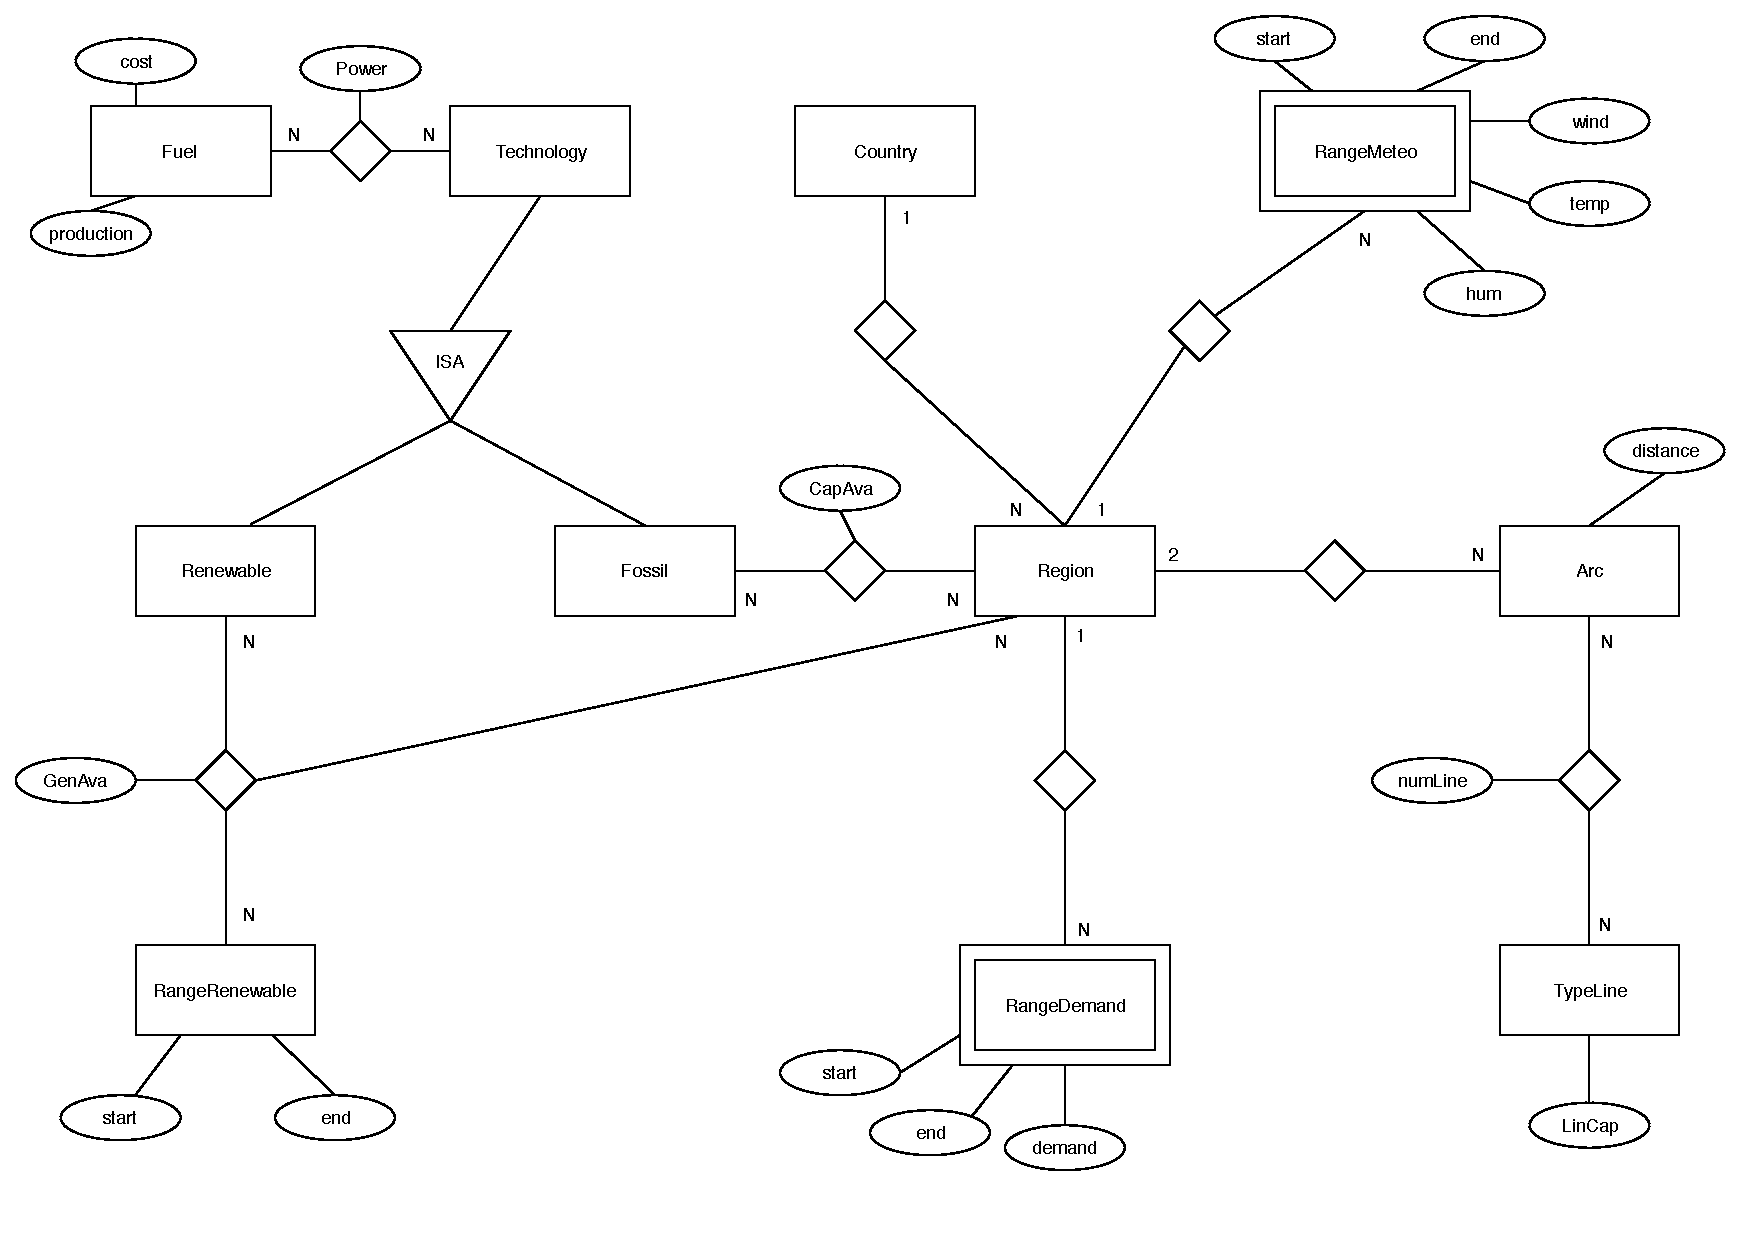
\includegraphics[width=1\textwidth]{/anexos/Diseno/DiagramaER}
	\caption{Diagrama entidad relación en la versión 1.}
	\label{img:modeloER}
\end{figure}

\begin{figure}[h]
	\centering
	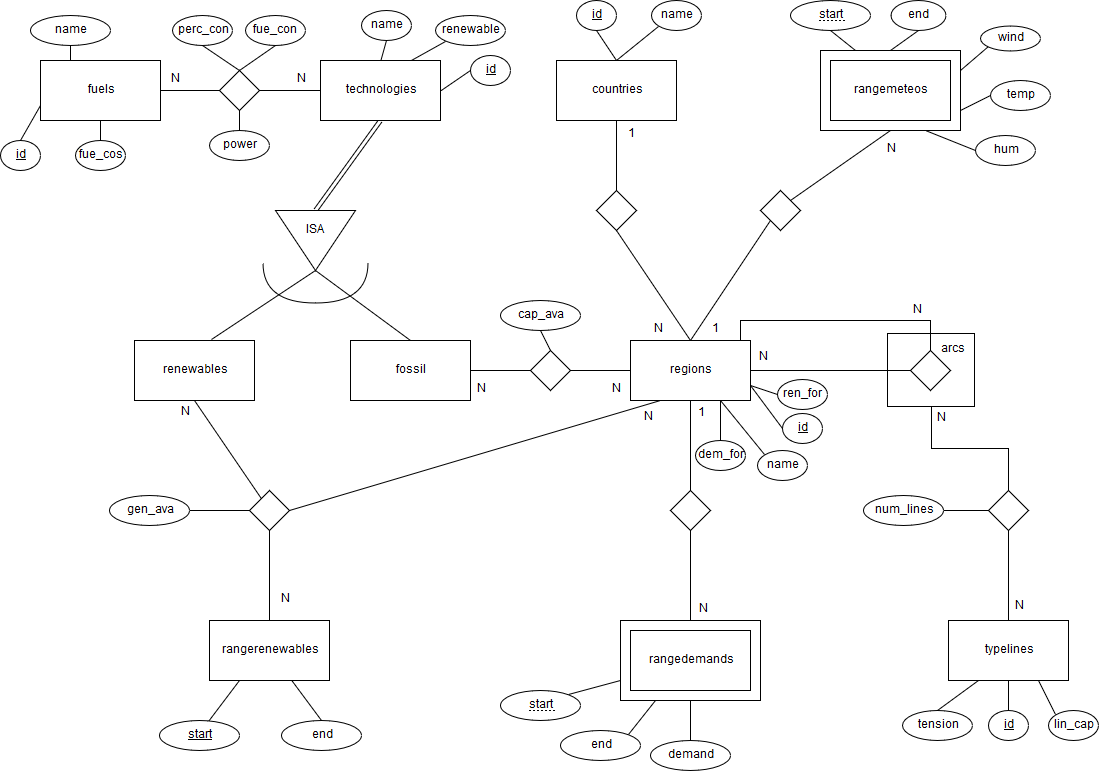
\includegraphics[width=1\textwidth]{/anexos/Diseno/DiagramaER2}
	\caption{Diagrama entidad relación en su versión 2.}
	\label{img:modeloER2}
\end{figure}

\begin{figure}[h]
	\centering
	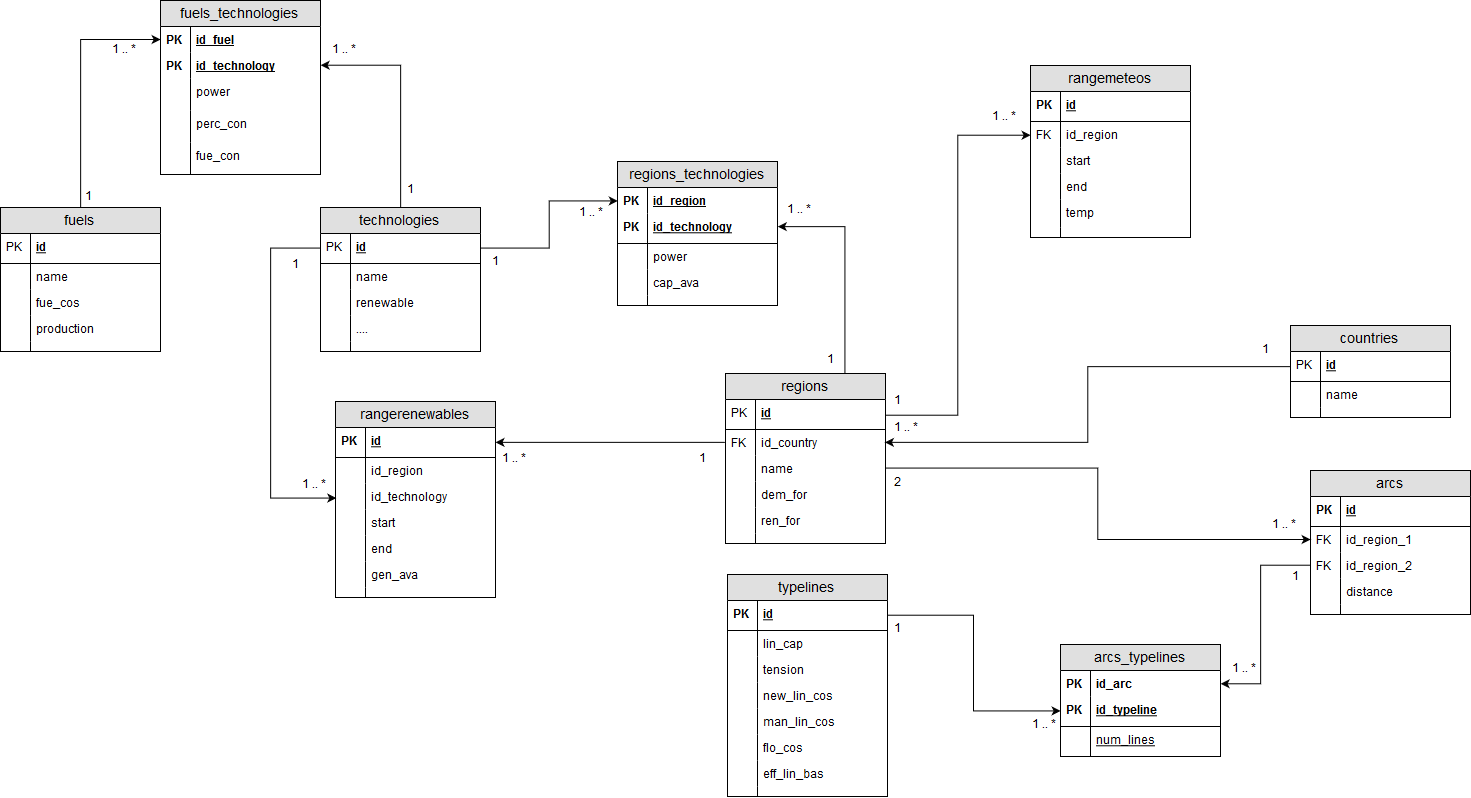
\includegraphics[width=1\textwidth]{/anexos/Diseno/DiagramaRelacional}
	\caption{Diagrama relacional.}
	\label{img:modeloRelacional}
\end{figure}

\newpage

\section{Diseño procedimental}

En esta sección se realizará un ejemplo de diagrama de secuencia para el caso de uso 1 que representa la actualización de datos mediante formularios. Concretamente, se representará la edición de una región. Podemos ver el diagrama de secuencia en la figura~\ref{img:modeloSecuencial}.

\begin{figure}[h]
	\centering
	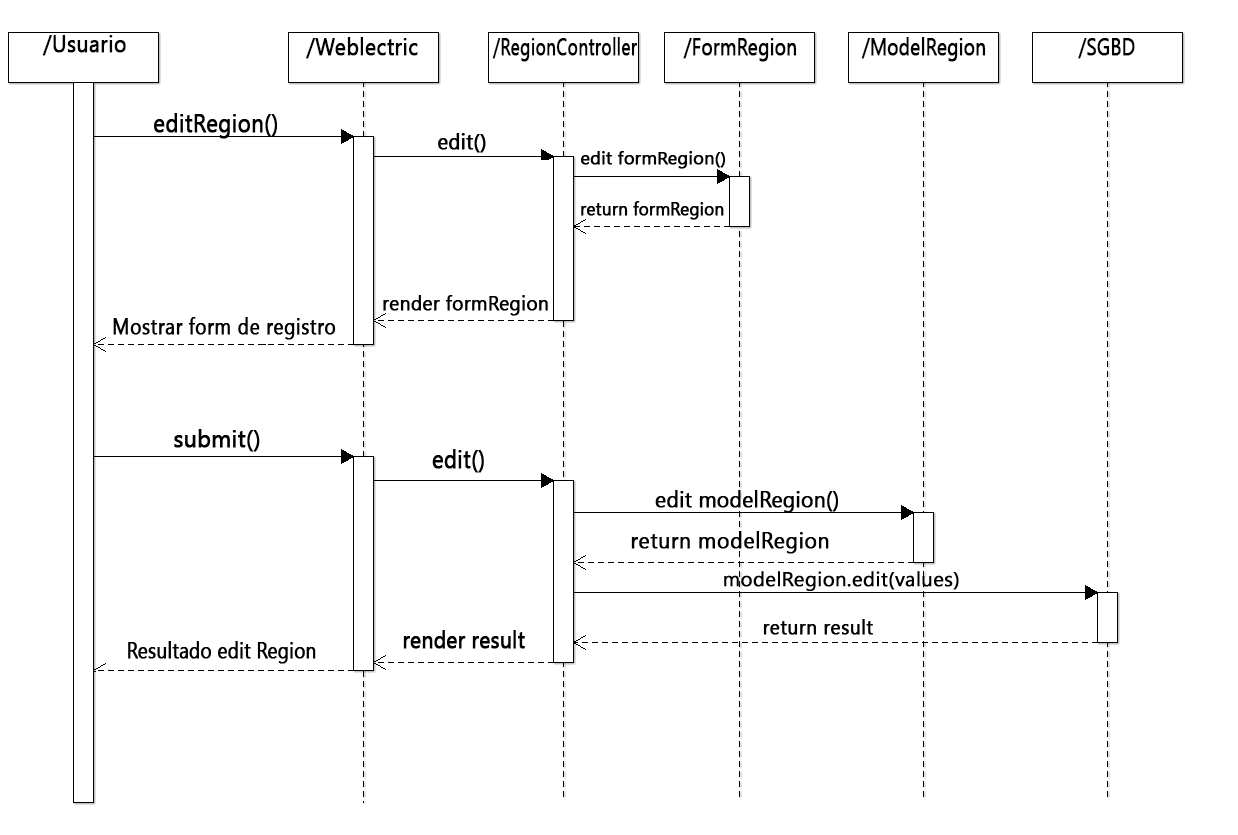
\includegraphics[width=1\textwidth]{/anexos/Diseno/DiagramaSecuencial}
	\caption{Diagrama secuencial del caso de uso 1: Administración mediante formularios.~\ref{tabla:cu1}.}
	\label{img:modeloSecuencial}
\end{figure}

\newpage

\section{Diseño arquitectónico}

En este apartado se va a comentar como está diseñada la aplicación.

Para el diseño de \textit{Weblectric} se ha seguido un patrón Modelo-Vista-Controlador~\ref{img:mvc}. Mediante este patrón, la aplicación queda completamente estructurada en tres secciones:

\begin{itemize}
	
	\item \textit{Modelo:} Se destinan a esta parte todas las funciones de interacción directa con la base de datos.
	
	\item \textit{Vista:} Aquí se guardan las pantallas que interactúan con el cliente.
	
	\item \textit{Controlador:} Aquí se encuentra la lógica de la aplicación. Hace de unión entre la vista y el modelo.

\end{itemize}

En la tabla~\ref{tabla:estructuraMVC} podemos ver qué directorio corresponde en nuestro proyecto a cada una de estas tres grandes secciones.

\begin{table}[h]
	\centering
	\caption{Estructura MVC en \textit{Weblectric}.}
	\label{tabla:estructuraMVC}
	\rowcolors {2}{gray!20}{}
	\begin{tabular}{p{5cm} p{5cm}}
		\toprule
		Patrón MVC 					 & Directorio en \textit{Weblectric}  \\ \midrule
		Modelos			        	 & \textit{models} 			    \\ 
		Vistas						 & \textit{templates}		    \\
		Controladores          		 & \textit{controllers}		 	\\ \bottomrule
	\end{tabular}
\end{table}

\begin{figure}[h]
	\centering
	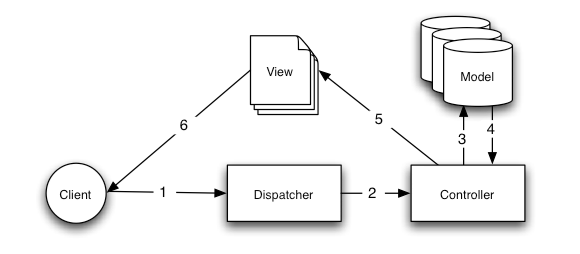
\includegraphics[width=1\textwidth]{/anexos/Diseno/mvc}
	\caption{Patrón Modelo-Vista-Controlador.~\cite{img:MVC}}
	\label{img:mvc}
\end{figure}

\newpage

Una vez conocida la estructura de la aplicación, mostraremos los pasos seguidos para construir las vistas. Dividiremos la clasificación en dos grupos: la idea inicial elaborada a través de unos \textit{mockups} y el resultado final.

\subsection{Mockups} 

El primer paso fue diseñar una plantilla (\textit{layout}). Esta plantilla, que se puede ver en la figura~\ref{img:layout} es común a todas las vistas.

Posteriormente, pasamos a diseñar la pantalla principal~\ref{img:home}. Aquí se iban a listar todas las entidades para que el usuario pudiese acceder a administrarlas.

Como se puede ver en la figura~\ref{img:home}, al pasar el ratón por encima, aparecerá una pequeña animación diferenciando cada una de las entidades. La siguiente pantalla que se va a presentar es la administración. Se tienen dos tipos de administraciones, las que son a partir de formularios y las que son mediante la subida de una hoja de cálculo. Pulsando en una de las entidades, nos iremos a su pantalla principal, a cada entidad la que le corresponda. 

\subsubsection{Administración mediante formularios} 

En la figura~\ref{img:entidadHome}, podemos ver la pantalla de administración de las entidades que utilizan formularios. En esta vista podremos hacer las siguientes acciones:

\begin{itemize}
	\item Crear un nuevo elemento:~\ref{img:entidadNew}.
	\item Editar un elemento existente:~\ref{img:entidadEdit}.
	\item Visualizar detalles de un elemento existente:~\ref{img:entidadView}.
	\item Eliminar un elemento:~\ref{img:entidadDelete}.
\end{itemize}

\subsubsection{Administración mediante hojas de cálculo} 

Como ya hemos comentado, hay algunas entidades que se administran a través de hojas de cálculo. En la figura~\ref{img:entidadExcel} encontramos un ejemplo. Además, existe la posibilidad de poder descargar una plantilla con todos los datos actuales, podemos modificar los datos y subir el fichero. 

\newpage

\subsection{Resultado final} 

Una vez presentados los mockups, comentaremos los cambios que se han ido produciendo a raíz de proposiciones del cliente y mejoras personales que hemos ido realizando durante el desarrollo.

La plantilla de la aplicación ha sufrido modificaciones pues además de añadir un logotipo personalizado para \textit{Weblectric}, se ha tenido que incluir una nueva funcionalidad, un botón para restablecer la base de datos a su situación inicial. Estos cambios se contemplan en la figura~\ref{img:Flayout}.

Puesto que las etiquetas de los campos de los formularios no tienen un nombre representativo, se ha decidido añadir un título a cada una de las etiquetas del formulario con la finalidad de aportar información acerca del significado del campo. Además, como resultaba de interés conocer qué usuario ha iniciado sesión en la aplicación, se creó en la cabecera una nueva sección. Por último, para facilitar la navegación por la aplicación, se han creado migas de pan. Todos estos resultados pueden verse en la figura~\ref{img:Ftooltips}.

Sin embargo, el cambio más significativo viene dado en la pantalla principal. Una vez enseñado el resultado al cliente, nos mandó reestructurar la forma en que distribuimos cada una de las entidades. Actualmente, ya no se representan así, sino que existen diferentes agrupaciones, cada una con su color y animación identificativos.

La estructura de la aplicación, con los cambios aplicados, queda de la siguiente manera:

\begin{itemize}
	
	\item Un primer grupo con tres pestañas~\ref{img:Fhome}:
	
	\begin{itemize}
		
		\item Countries data: \ref{img:Fcountries}. 
		
		\begin{itemize}
			
			\item Country.
			\item Renewable source.
			\item Climate.
			\item Current System.
			
		\end{itemize}
		
		\item Technologies:\ref{img:Ftechnologies}.
		
		\begin{itemize}
			
			\item Generation technologies.
			\item Types of lines.
			\item Fuels.
			
		\end{itemize}
		
		\item Simulation: \ref{img:Fsimulation}.
		
		\begin{itemize}
			
			\item Objectives.
			\item Download.
			
		\end{itemize}
	
		\item Users: \ref{img:Fusers}.
		
	\end{itemize}
	
\end{itemize}

A continuación, siguiendo con el mismo criterio que en el apartado de los \textit{mockups}, mostraremos las imágenes clasificando los dos tipos de administraciones

\subsubsection{Administración mediante formularios} 

Cogiendo como ejemplo la entidad "technologies", los resultados son: 

\begin{itemize}
	\item Pantalla principal de esa entidad~\ref{img:FentidadHome}.
	\item Crear una nueva tecnología:~\ref{img:FentidadNew}.
	\item Editar una tecnología:~\ref{img:FentidadEdit}.
	\item Visualizar detalles de una tecnología:~\ref{img:FentidadView}.
	\item Eliminar una tecnología:~\ref{img:FentidadDelete}.
\end{itemize}

\subsubsection{Administración mediante hojas de cálculo} 

En la figura~\ref{img:FentidadExcel} encontramos un ejemplo de como se administran los datos climáticos. 

\subsubsection{Administración de usuarios} 

En la figura~\ref{img:Fusersform} encontramos un ejemplo de como se administran los usuarios. En este caso, el ejemplo es de la acción editar. 

\subsubsection{Simulación y exportación de ficheros} 

En la figura~\ref{img:Fobjectives}, habiendo pulsado sobre el icono de objetivos, se encuentran diferentes opciones. Los objetivos están clasificados en tres grandes bloques. Marcando las casillas, el valor se guardará en sesión y se podrá exportar desde la pantalla de descargas situada dentro de simulación.

En la figura~\ref{img:Fsimulationdownloads} se puede ver un listado con las simulaciones generadas, además se podrá crear una nueva y establecer el nombre deseado, figura~\ref{img:Fsimulationname}.

%MOCKUPS:

\begin{figure}[h]
	\centering
	
\includegraphics[width=1\textwidth]{/anexos/Diseno/Mockups/layout}
	\caption{Mockup: Plantilla común a todas las vistas.}
	\label{img:layout}
\end{figure}

\begin{figure}[h]
	\centering
	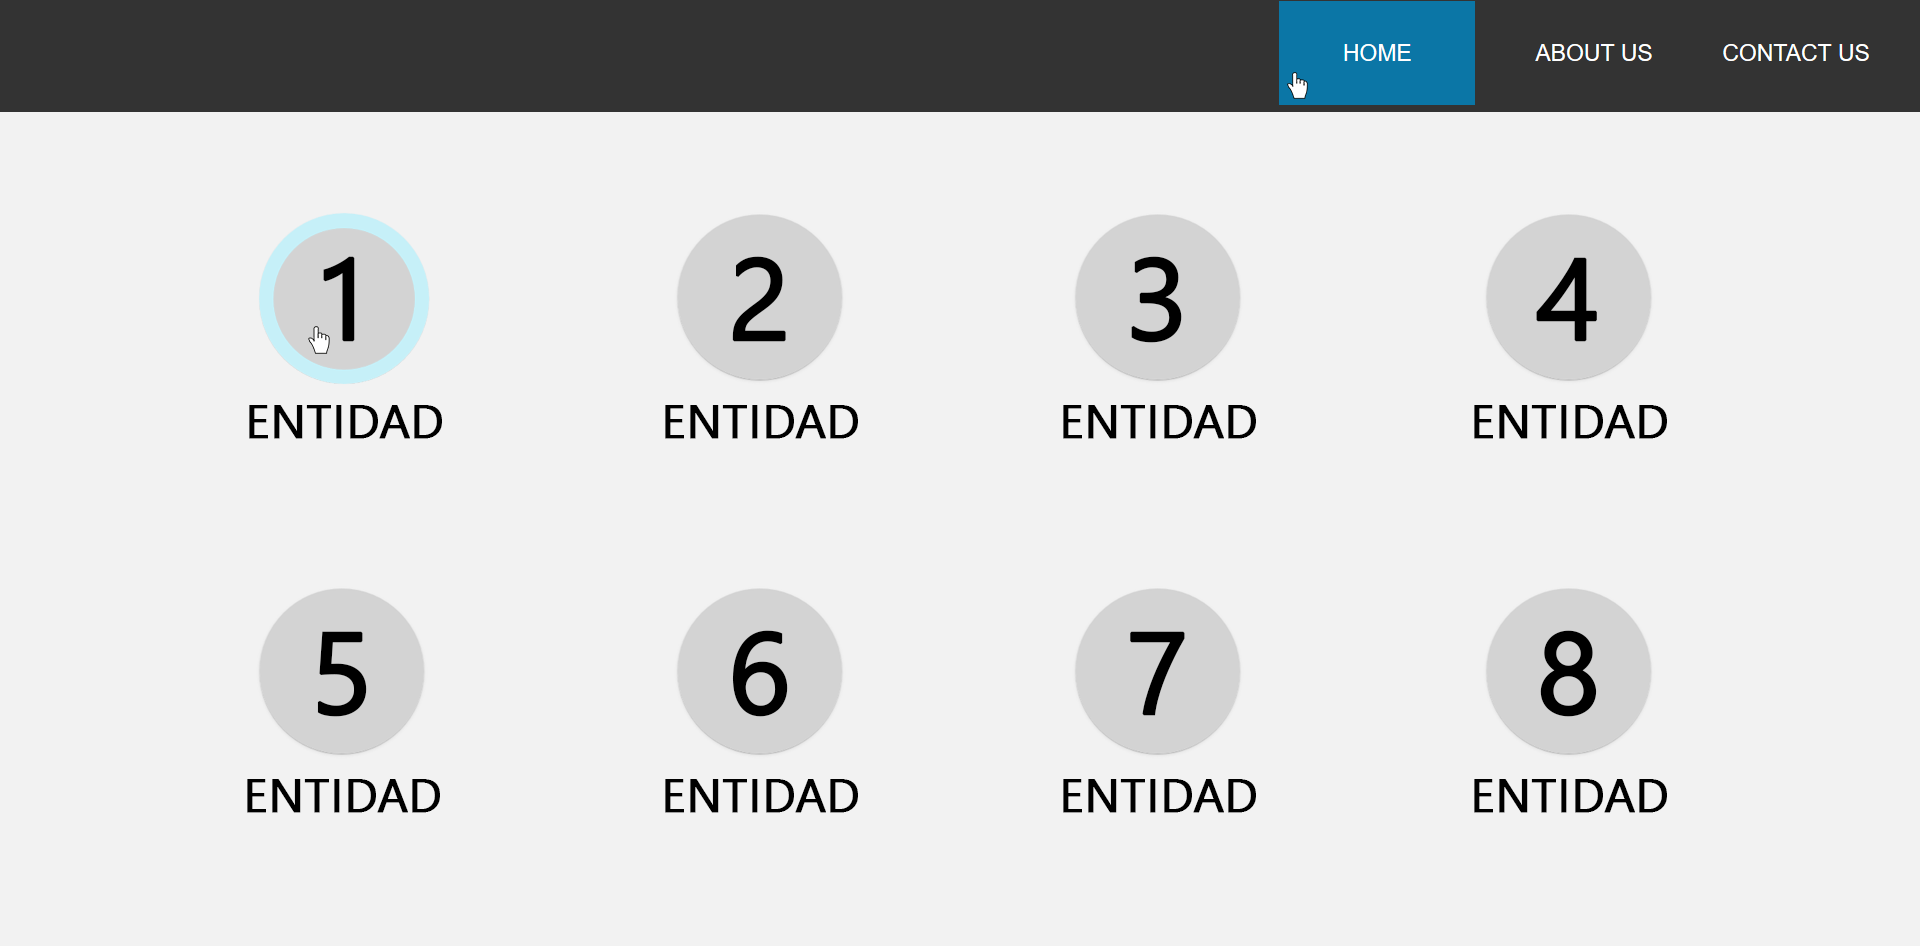
\includegraphics[width=1\textwidth]{/anexos/Diseno/Mockups/home}
	\caption{Mockup: Pantalla principal.}
	\label{img:home}
\end{figure}

\begin{figure}[h]
	\centering
	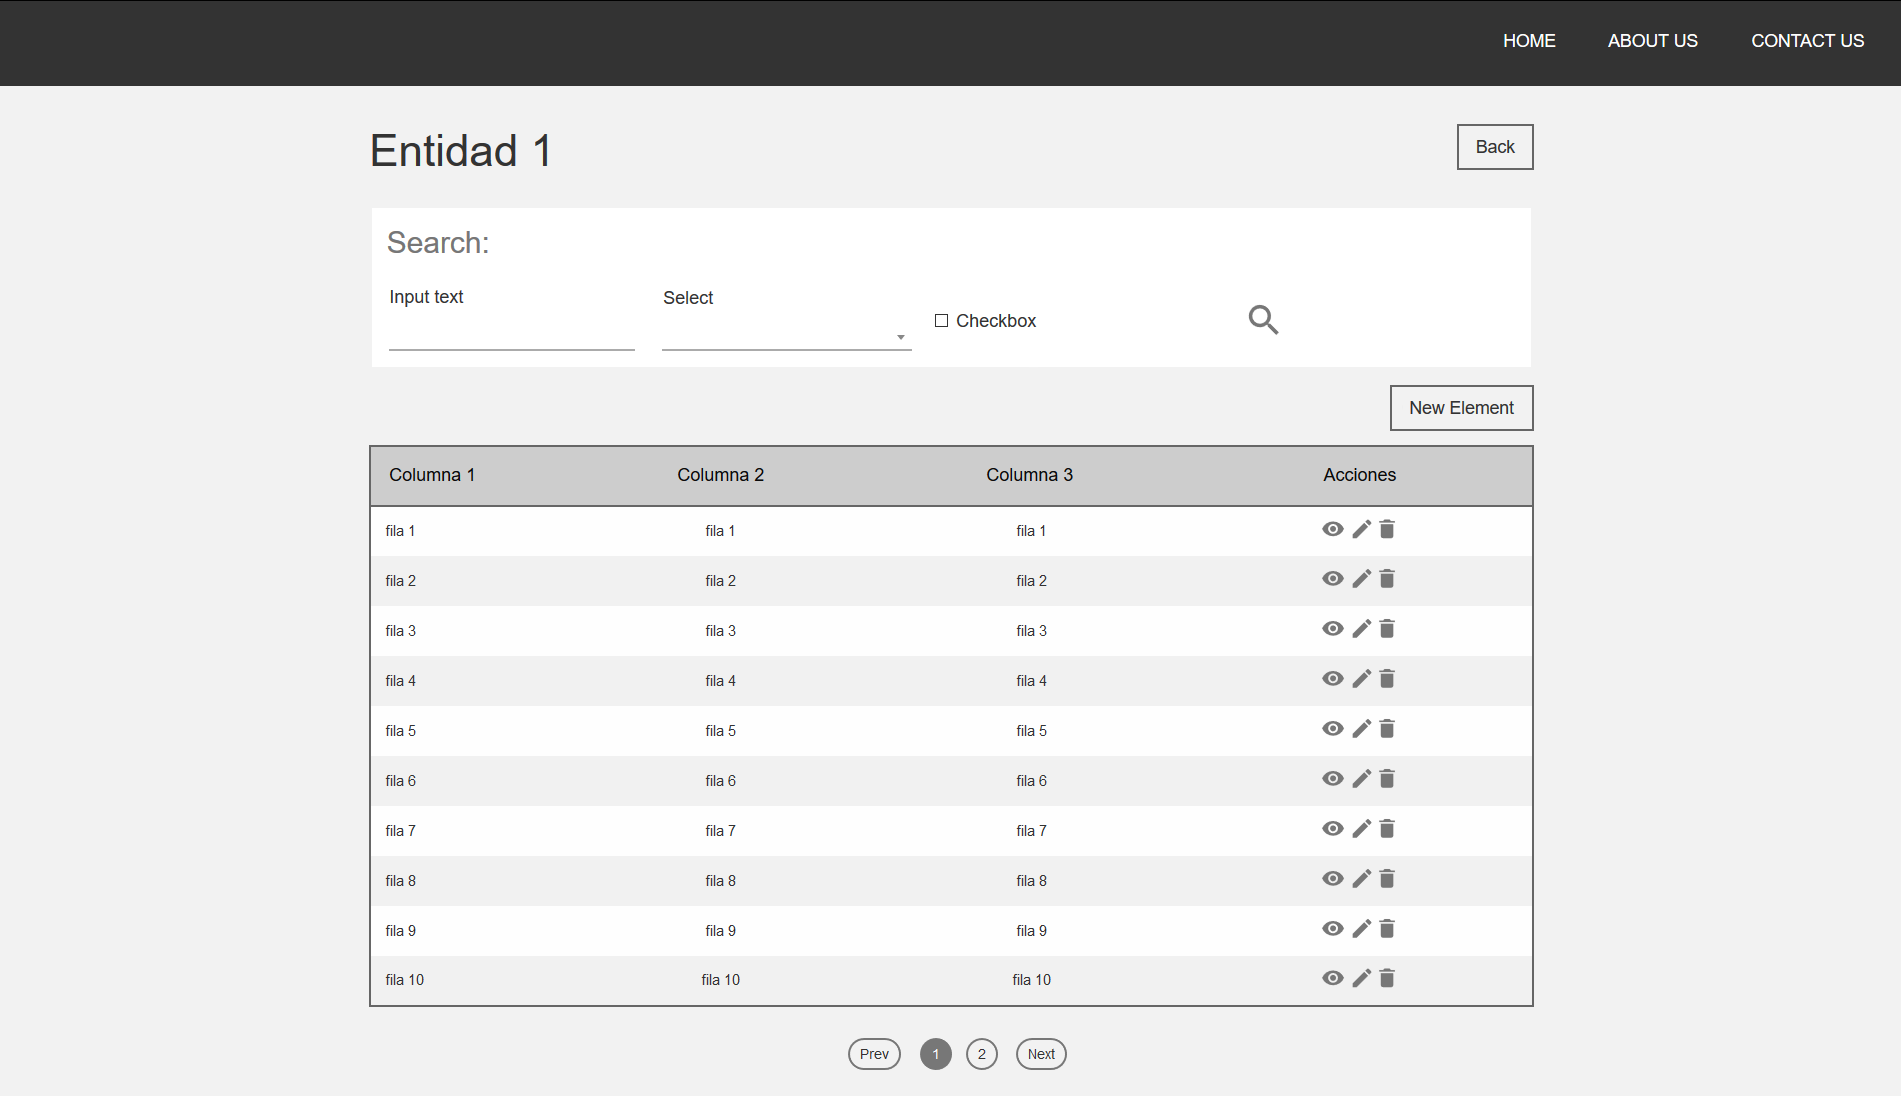
\includegraphics[width=1\textwidth]{/anexos/Diseno/Mockups/entidadHome}
	\caption{Mockup: Pantalla principal de la entidad 1.}
	\label{img:entidadHome}
\end{figure}

\begin{figure}[h]
	\centering
	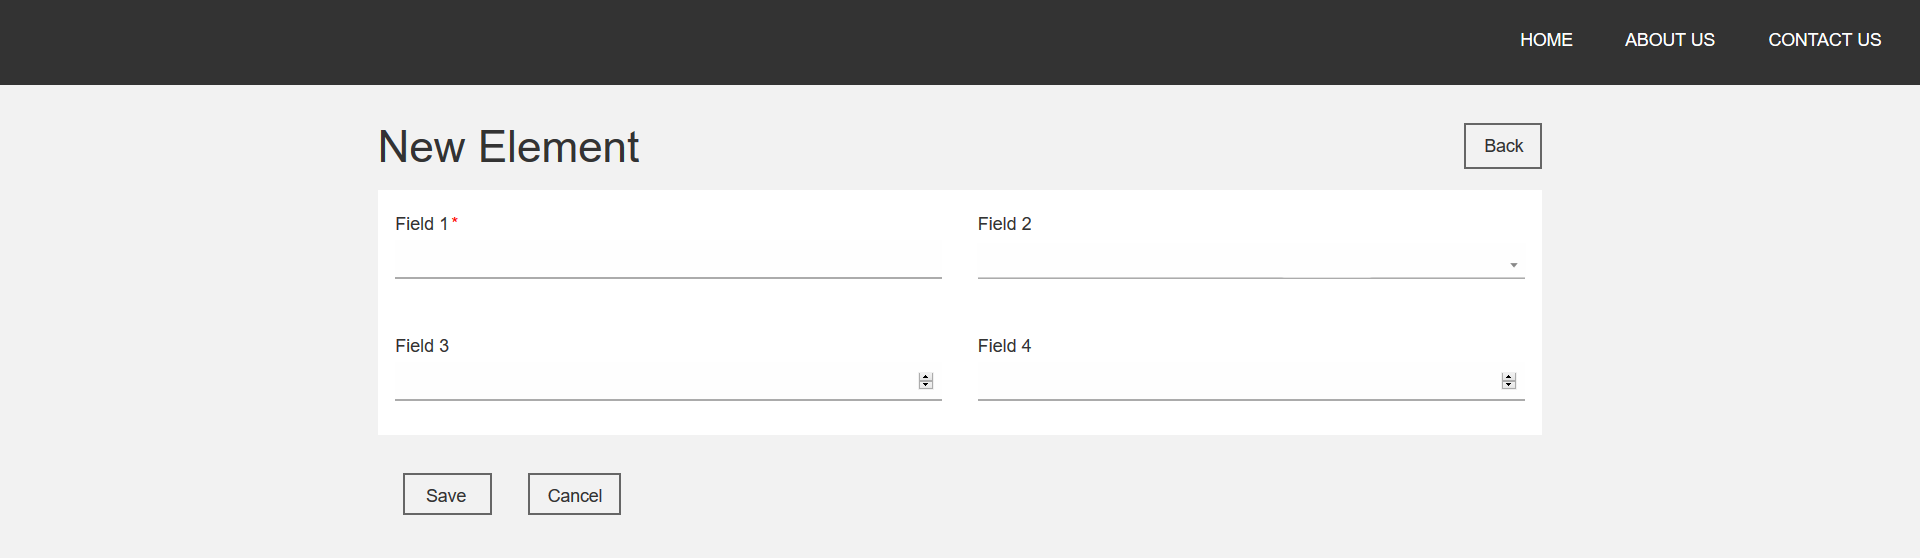
\includegraphics[width=1\textwidth]{/anexos/Diseno/Mockups/entidadNew}
	\caption{Mockup: Alta de un elemento.}
	\label{img:entidadNew}
\end{figure}

\begin{figure}[h]
	\centering
	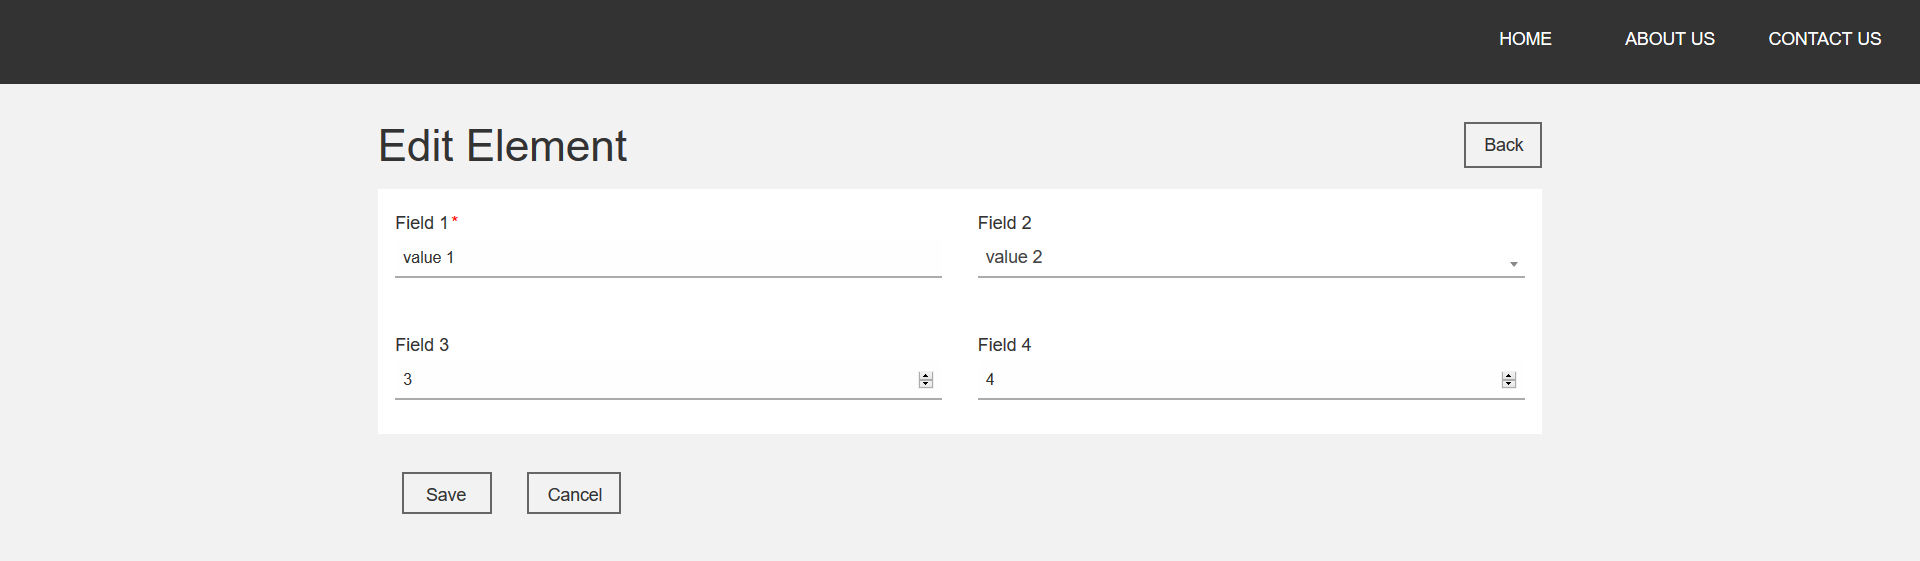
\includegraphics[width=1\textwidth]{/anexos/Diseno/Mockups/entidadEdit}
	\caption{Mockup: Edición de un elemento.}
	\label{img:entidadEdit}
\end{figure}

\begin{figure}[h]
	\centering
	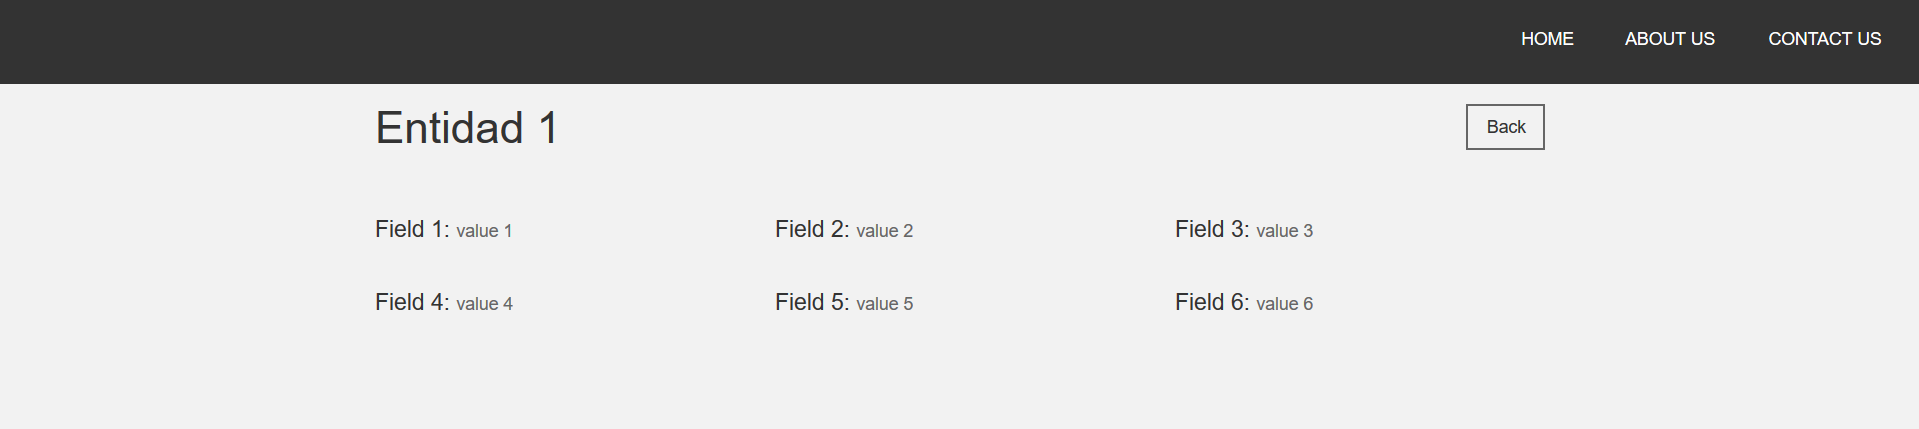
\includegraphics[width=1\textwidth]{/anexos/Diseno/Mockups/entidadView}
	\caption{Mockup: Visualización completa de un elemento.}
	\label{img:entidadView}
\end{figure}

\begin{figure}[h]
	\centering
	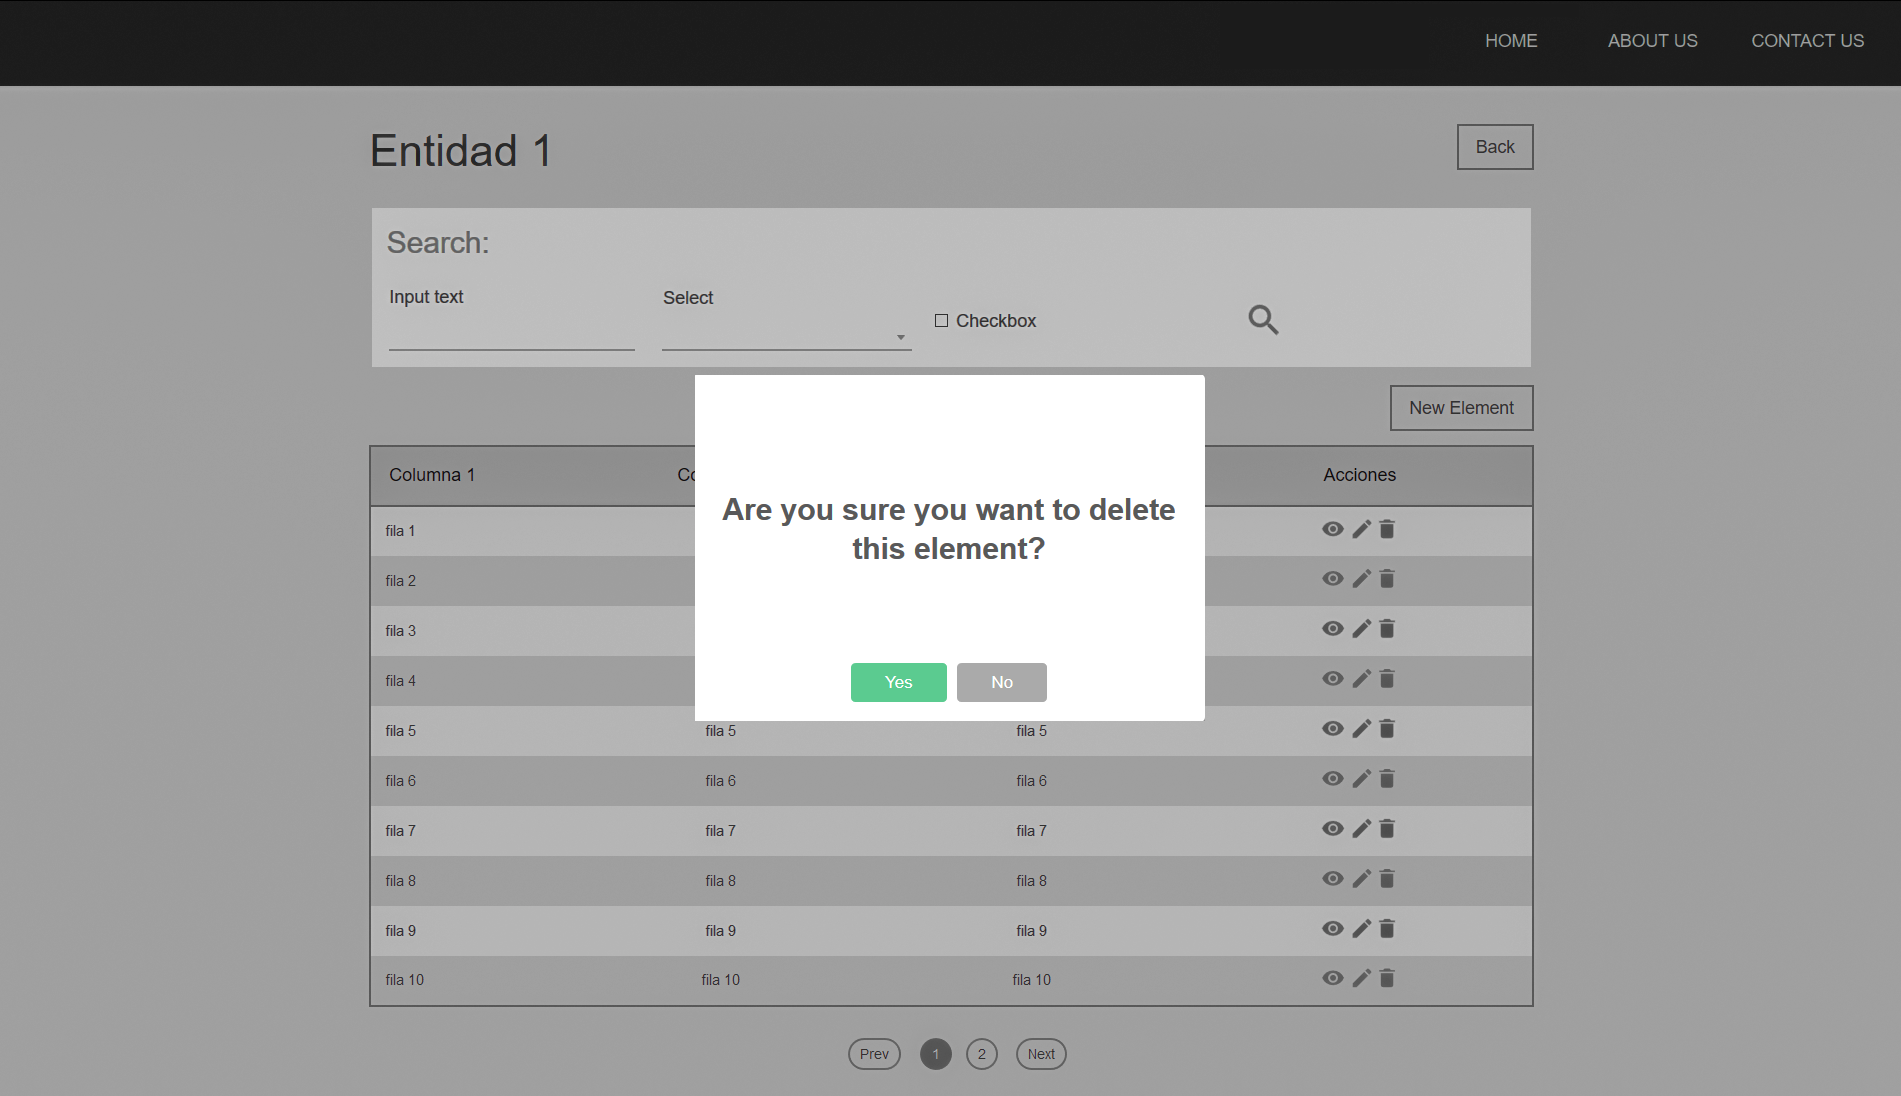
\includegraphics[width=1\textwidth]{/anexos/Diseno/Mockups/entidadDelete}
	\caption{Mockup: Mensaje de confirmación al eliminar un elemento.}
	\label{img:entidadDelete}
\end{figure}

\begin{figure}[h]
	\centering
	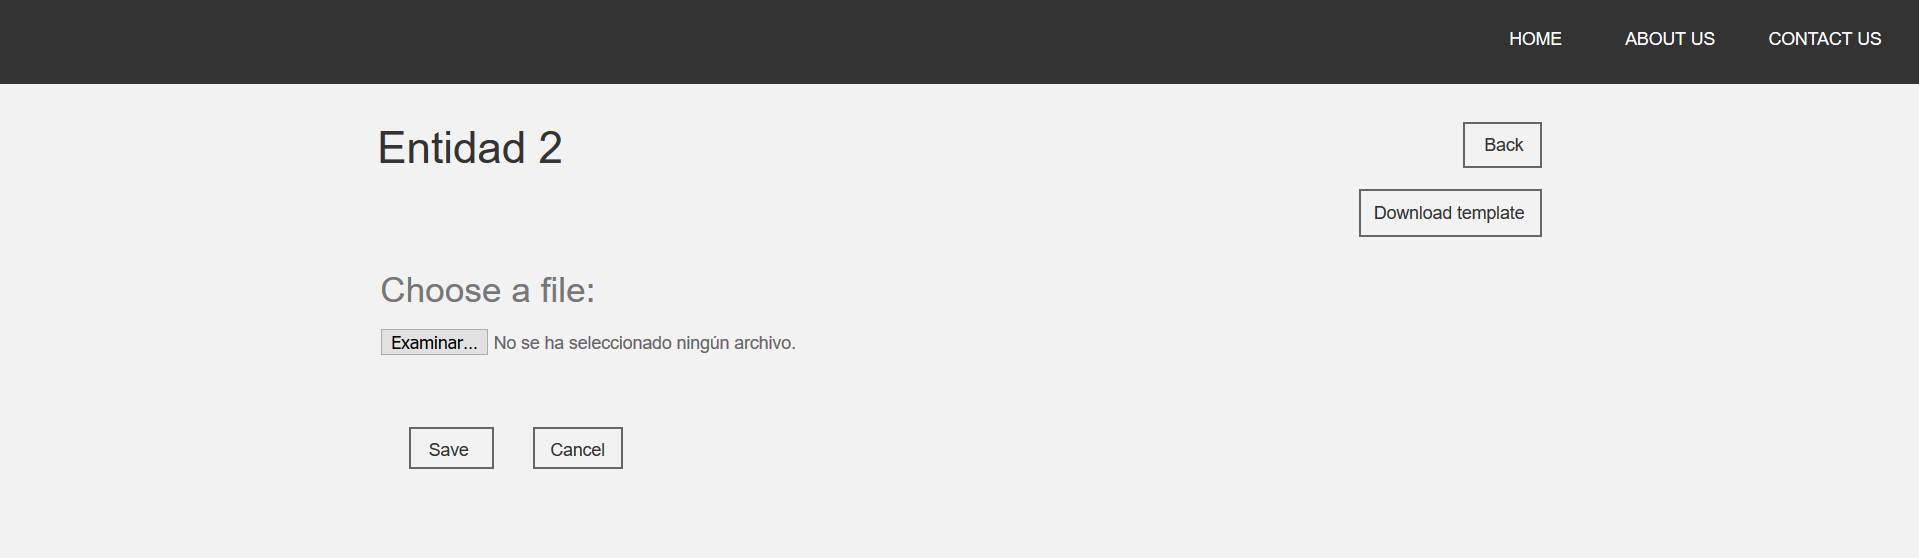
\includegraphics[width=1\textwidth]{/anexos/Diseno/Mockups/entidadExcel}
	\caption{Mockup: Administración de entidades mediante hoja de cálculo.}
	\label{img:entidadExcel}
\end{figure}

%RESULTADO FINAL:

\begin{figure}[h]
	\centering
	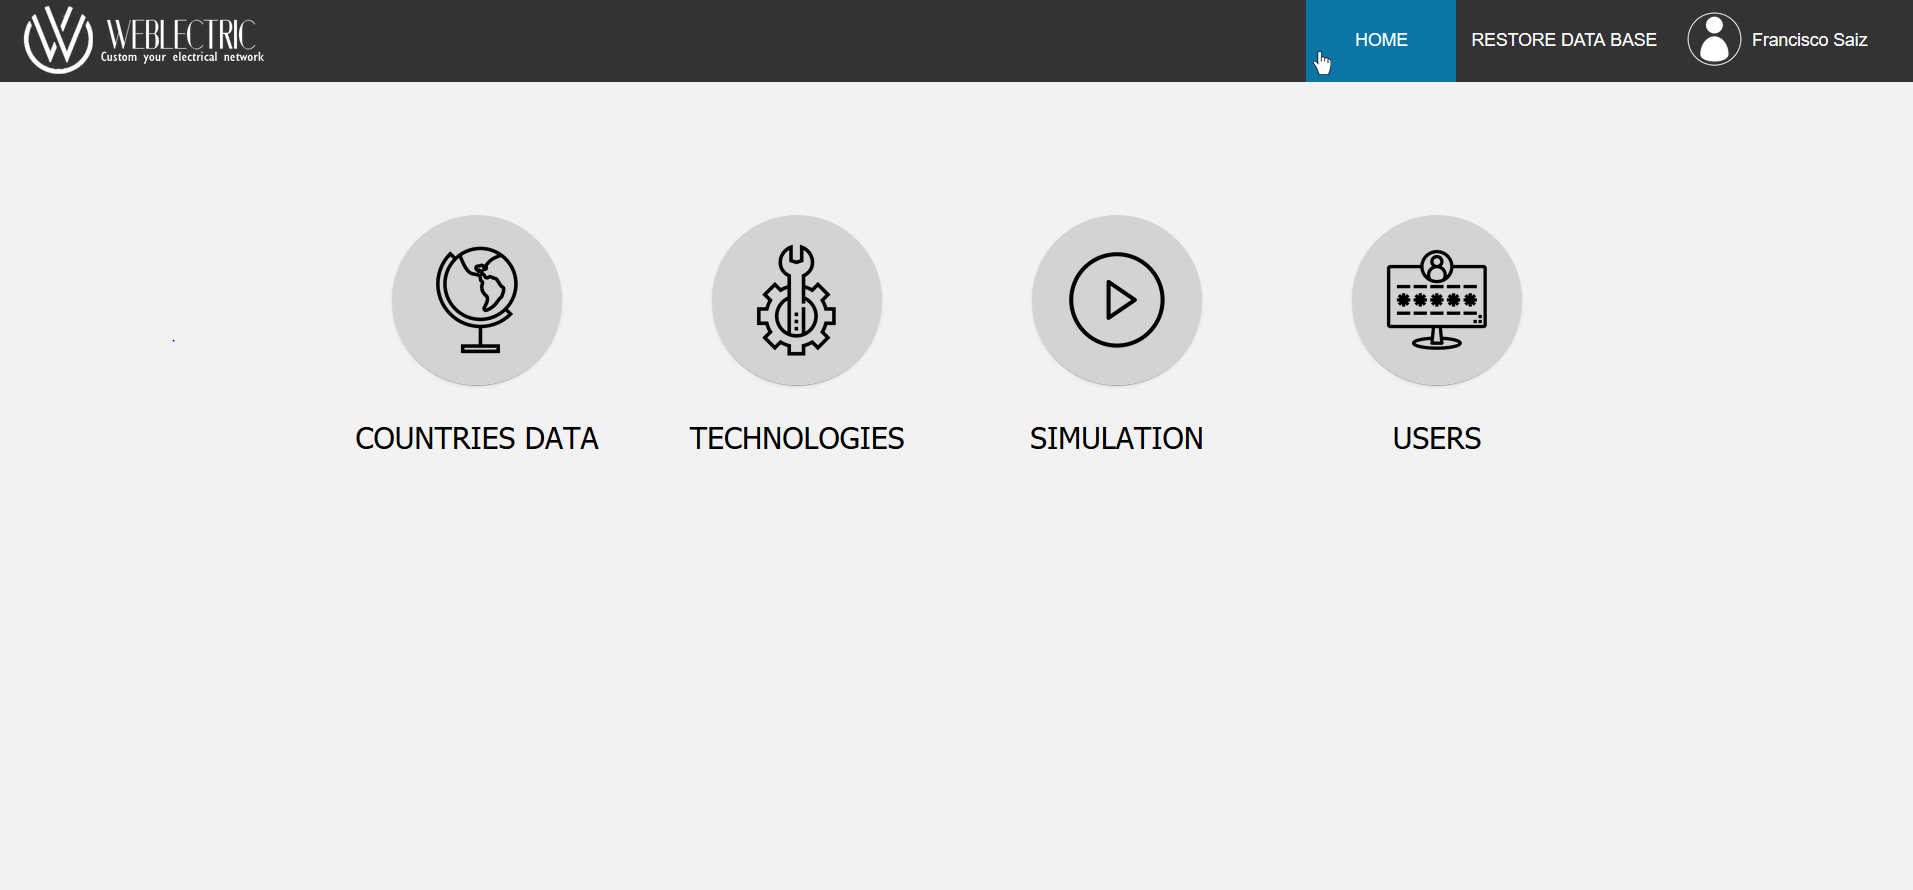
\includegraphics[width=1\textwidth]{/anexos/Diseno/Mockups/Flayout}
	\caption{Resultado final: Plantilla común a todas las vistas.}
	\label{img:Flayout}
\end{figure}

\begin{figure}[h]
	\centering
	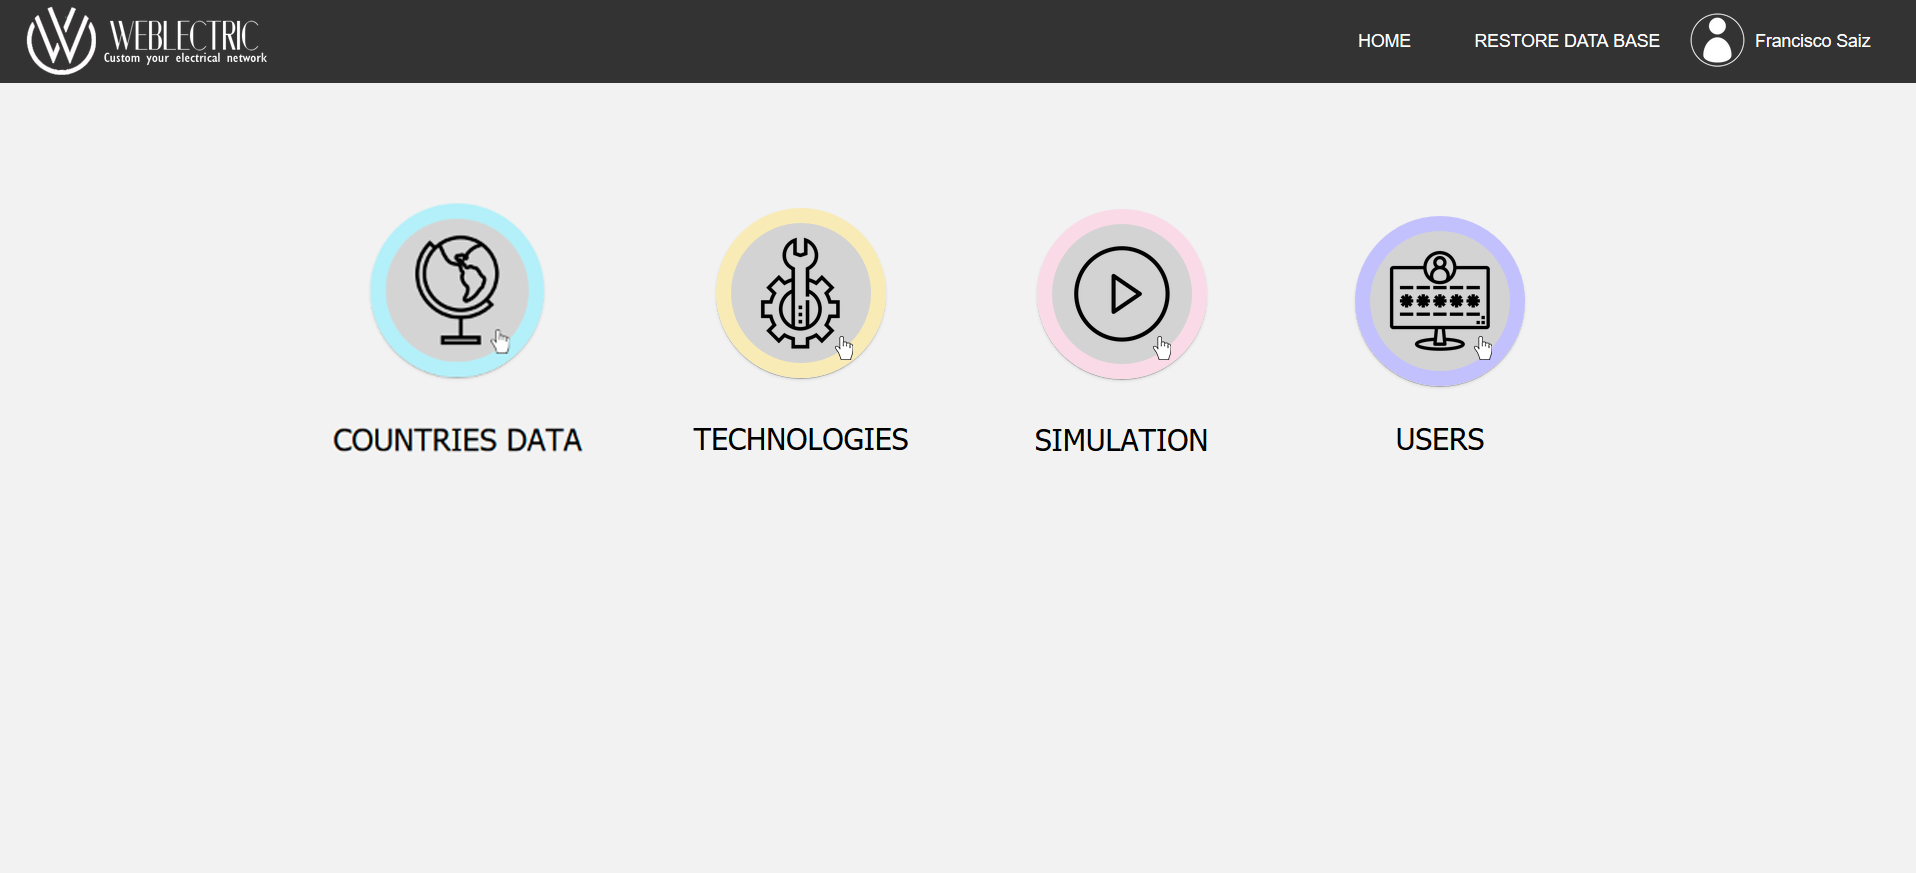
\includegraphics[width=1\textwidth]{/anexos/Diseno/Mockups/Fhome}
	\caption{Resultado final: Pantalla principal.}
	\label{img:Fhome}
\end{figure}

\begin{figure}[h]
	\centering
	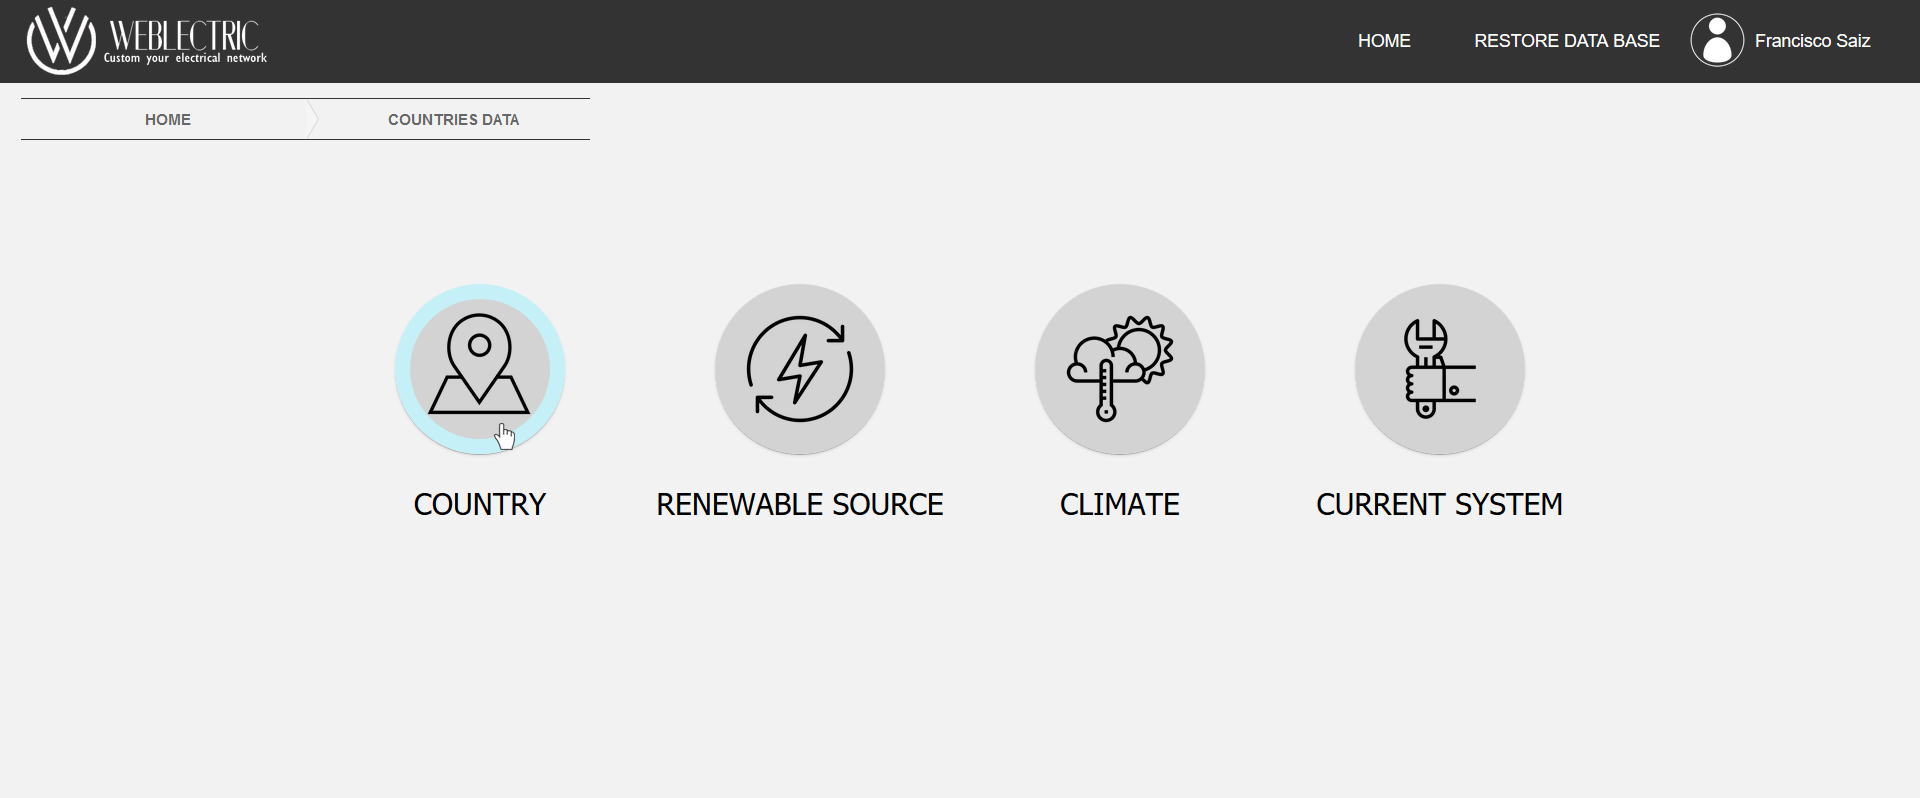
\includegraphics[width=1\textwidth]{/anexos/Diseno/Mockups/Fcountries}
	\caption{Resultado final: Pantalla países.}
	\label{img:Fcountries}
\end{figure}

\begin{figure}[h]
	\centering
	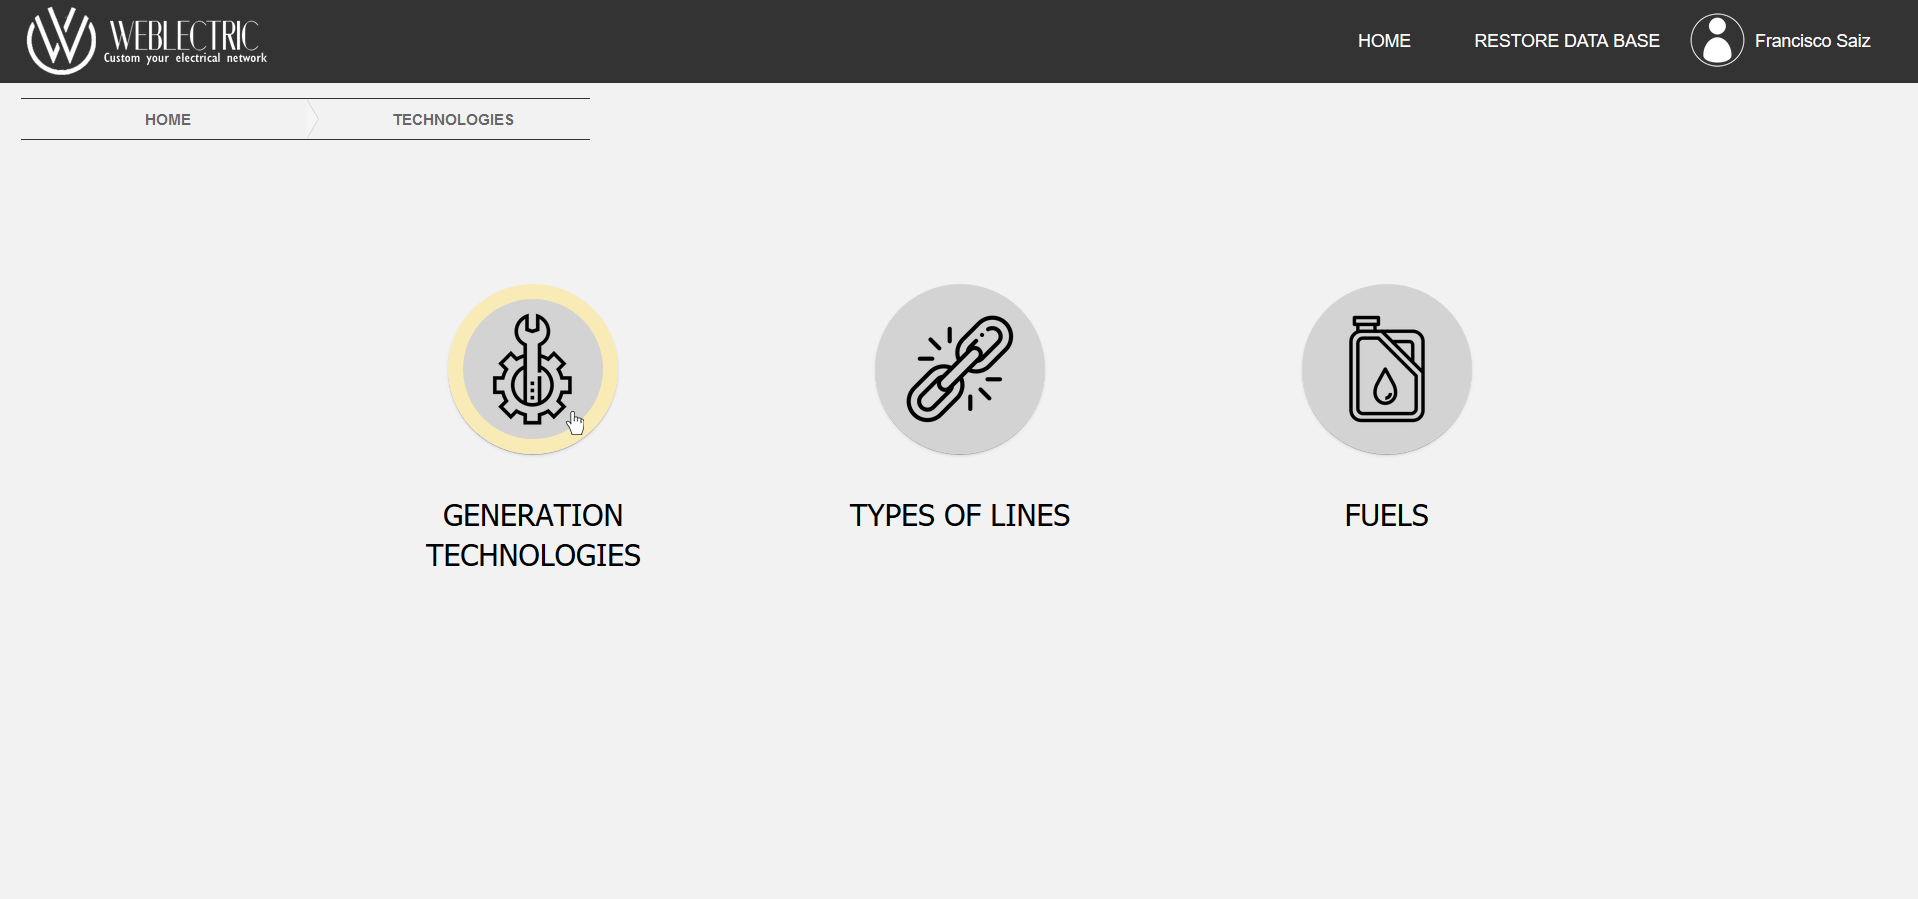
\includegraphics[width=1\textwidth]{/anexos/Diseno/Mockups/Ftechnologies}
	\caption{Resultado final: Pantalla tecnologías.}
	\label{img:Ftechnologies}
\end{figure}

\begin{figure}[h]
	\centering
	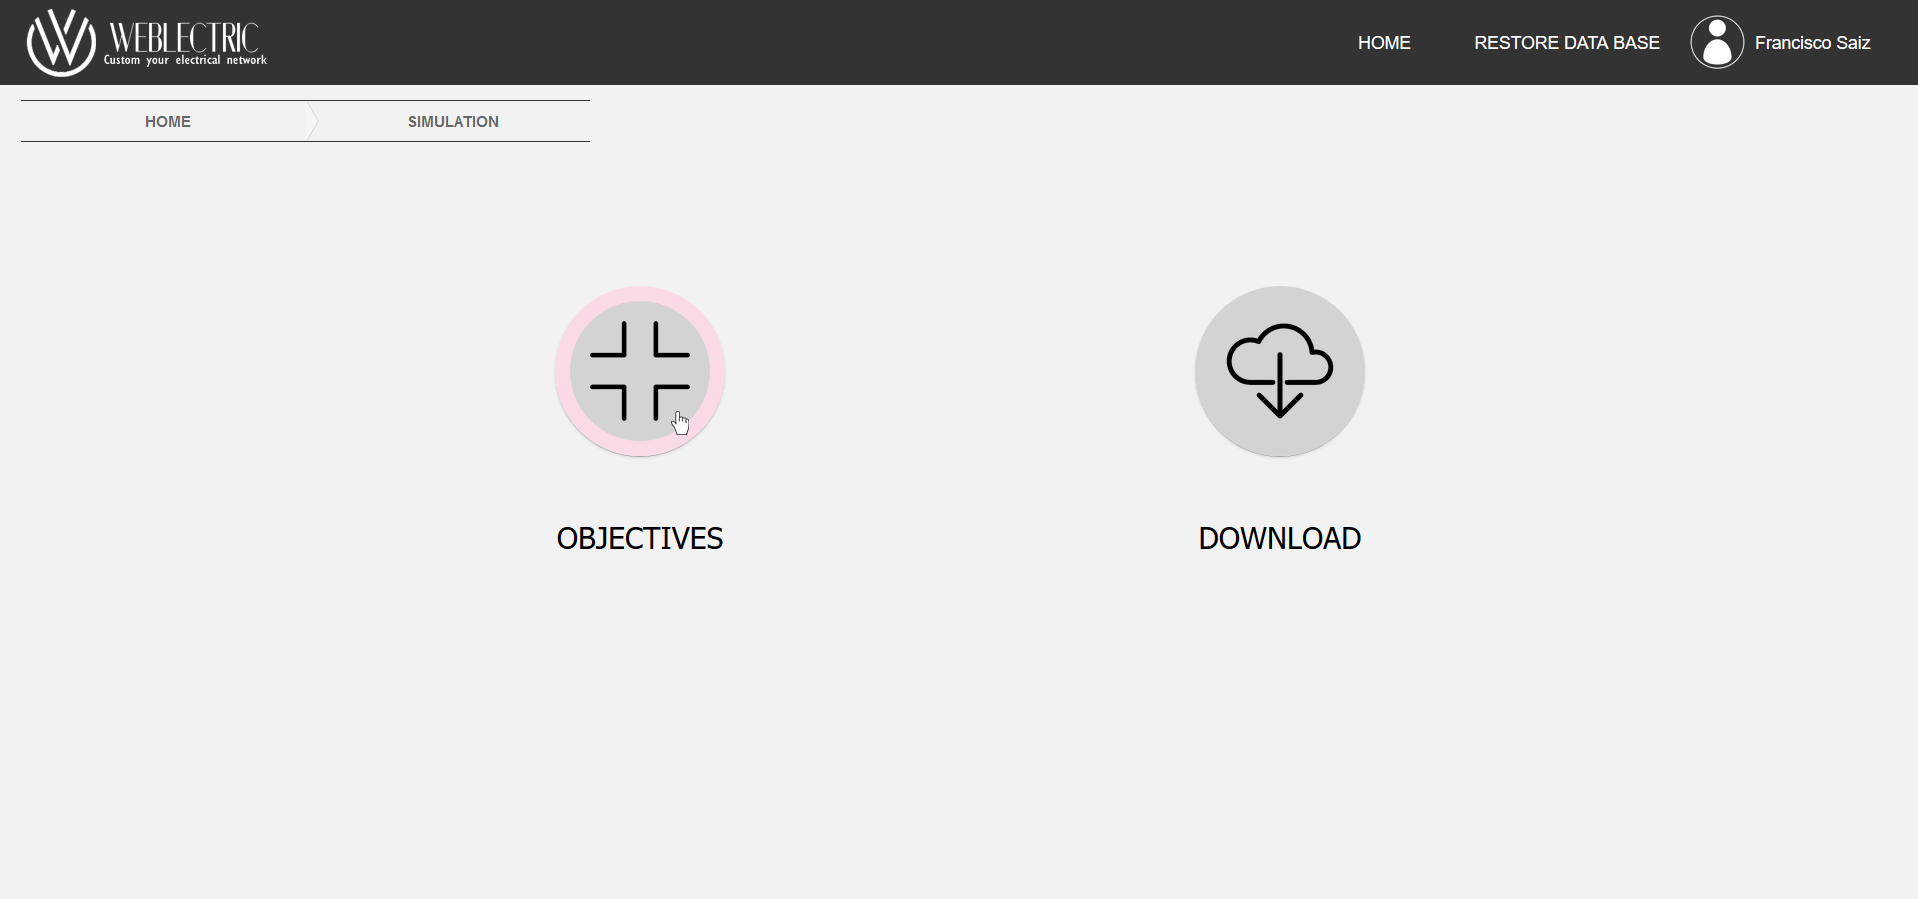
\includegraphics[width=1\textwidth]{/anexos/Diseno/Mockups/Fsimulation}
	\caption{Resultado final: Pantalla simulación.}
	\label{img:Fsimulation}
\end{figure}

\begin{figure}[h]
	\centering
	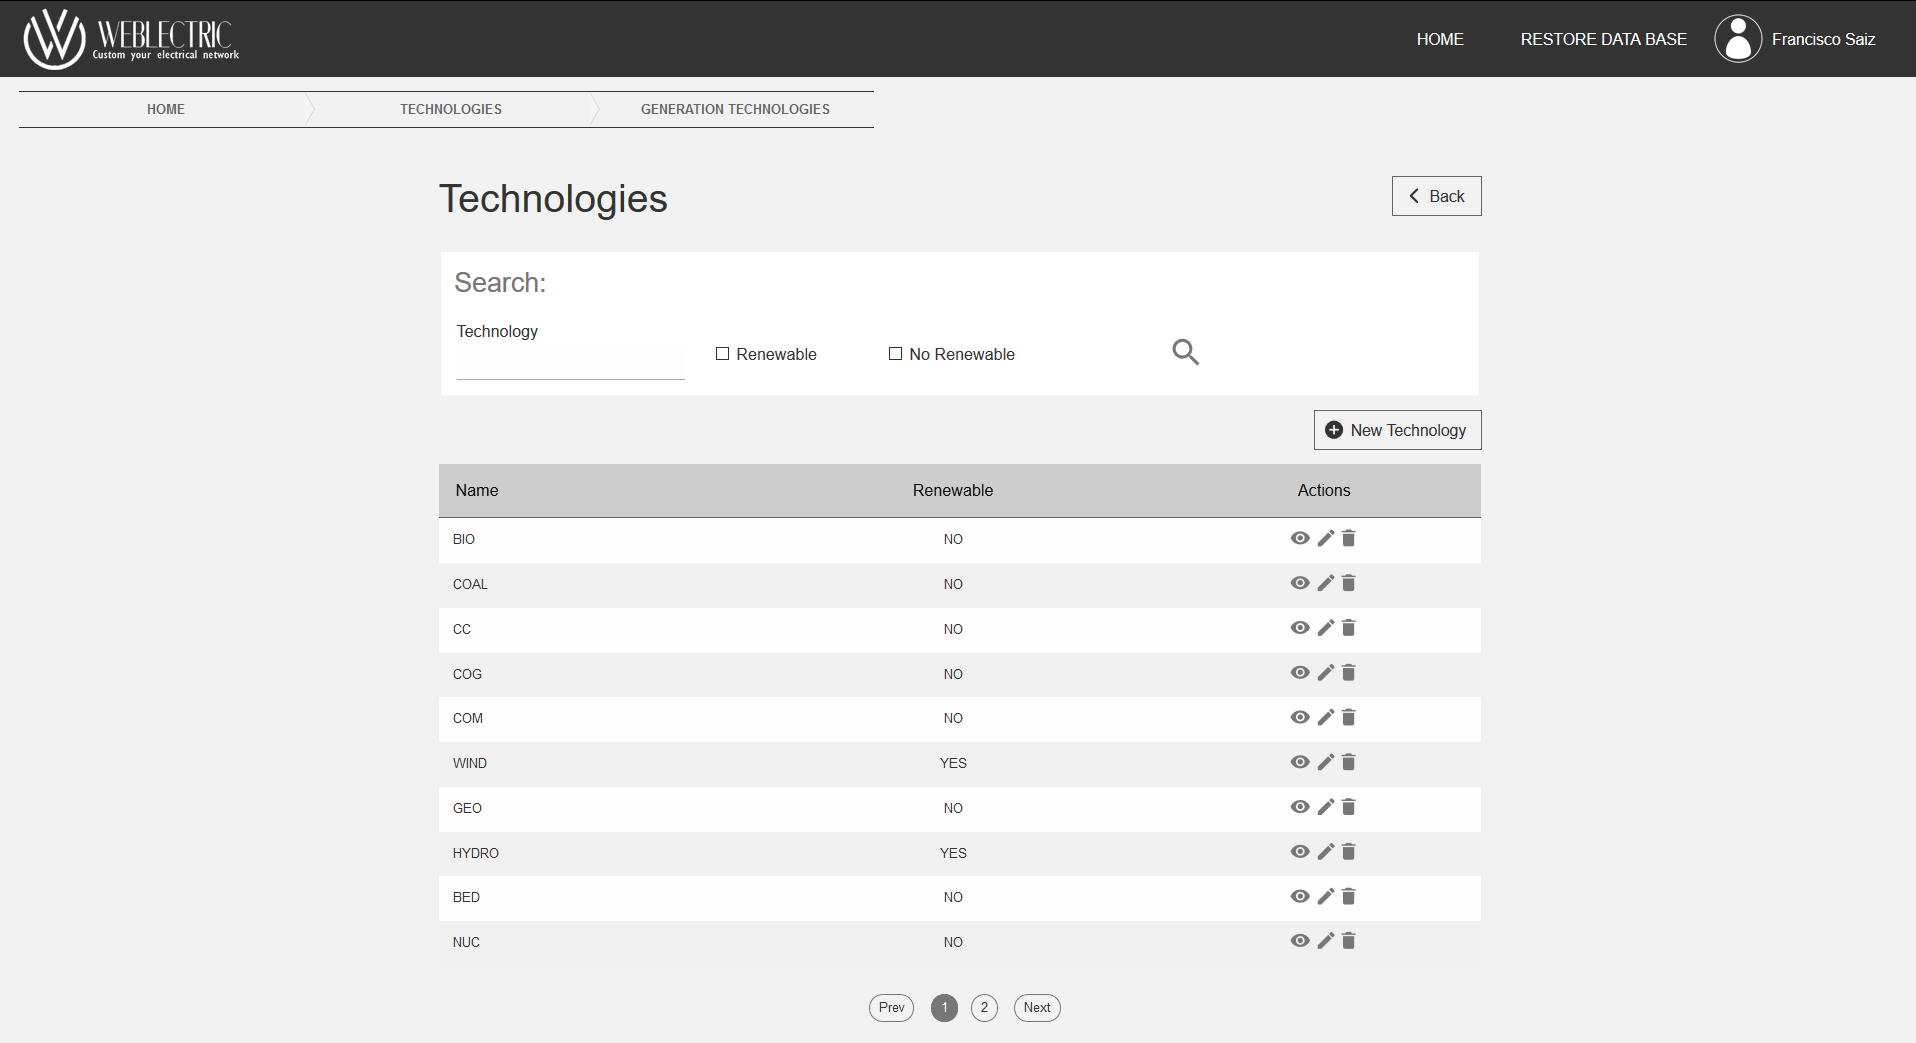
\includegraphics[width=1\textwidth]{/anexos/Diseno/Mockups/FentidadHome}
	\caption{Resultado final: Pantalla principal de la entidad Technology.}
	\label{img:FentidadHome}
\end{figure}

\begin{figure}[h]
	\centering
	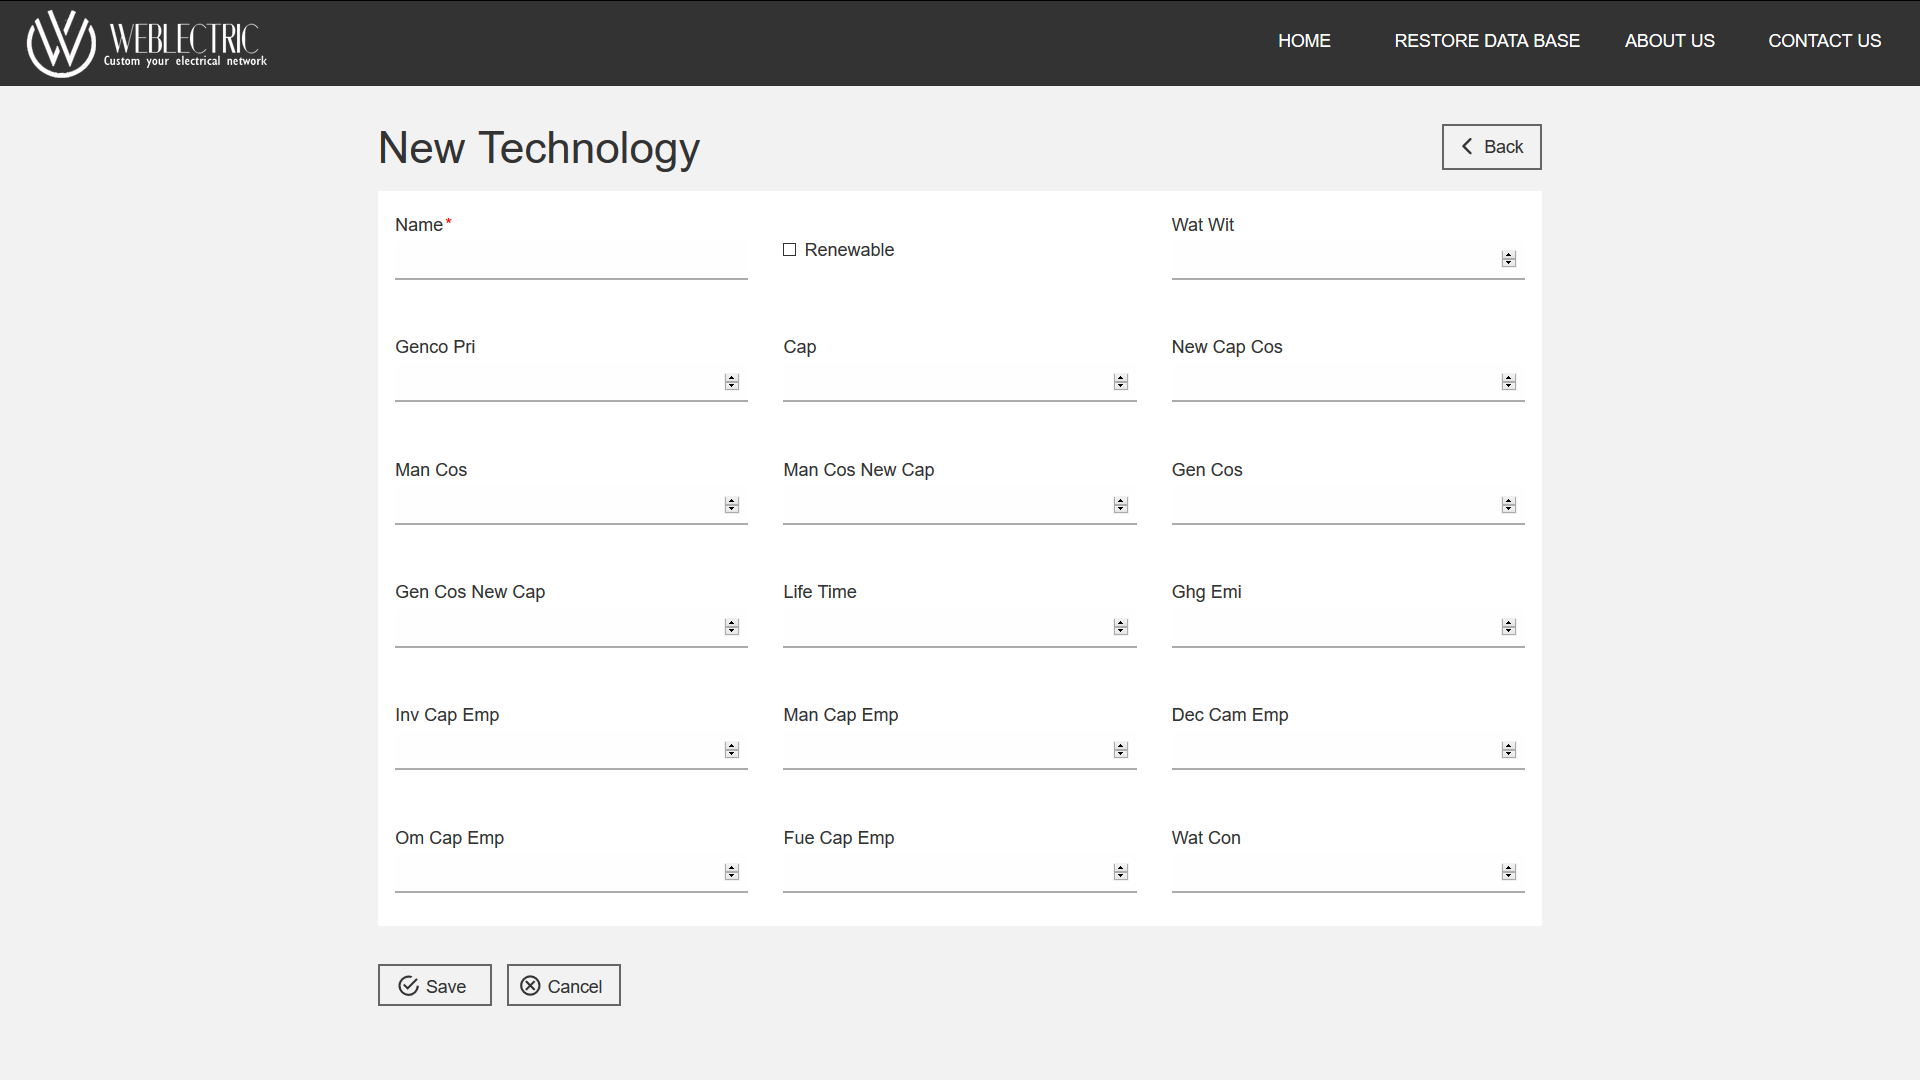
\includegraphics[width=1\textwidth]{/anexos/Diseno/Mockups/FentidadNew}
	\caption{Resultado final: Alta de un elemento.}
	\label{img:FentidadNew}
\end{figure}

\begin{figure}[h]
	\centering
	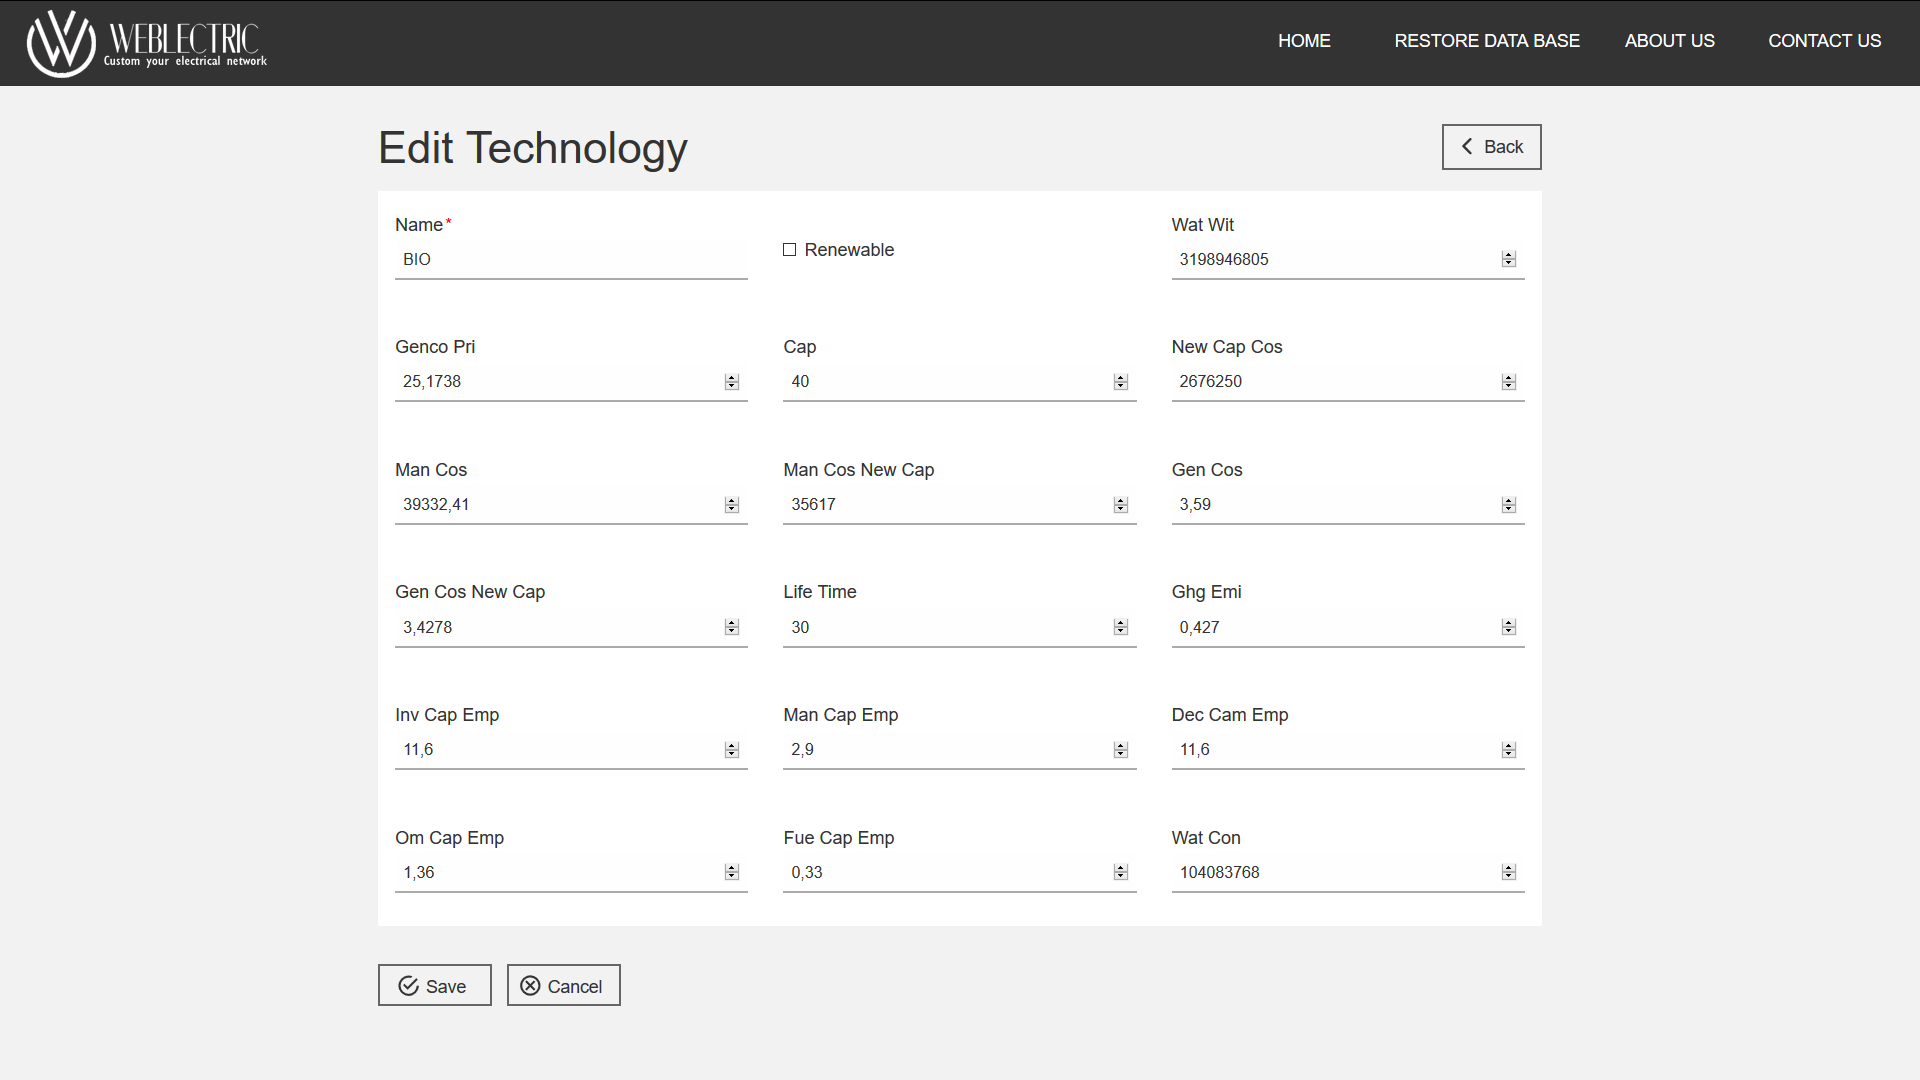
\includegraphics[width=1\textwidth]{/anexos/Diseno/Mockups/FentidadEdit}
	\caption{Resultado final: Edición de un elemento.}
	\label{img:FentidadEdit}
\end{figure}

\begin{figure}[h]
	\centering
	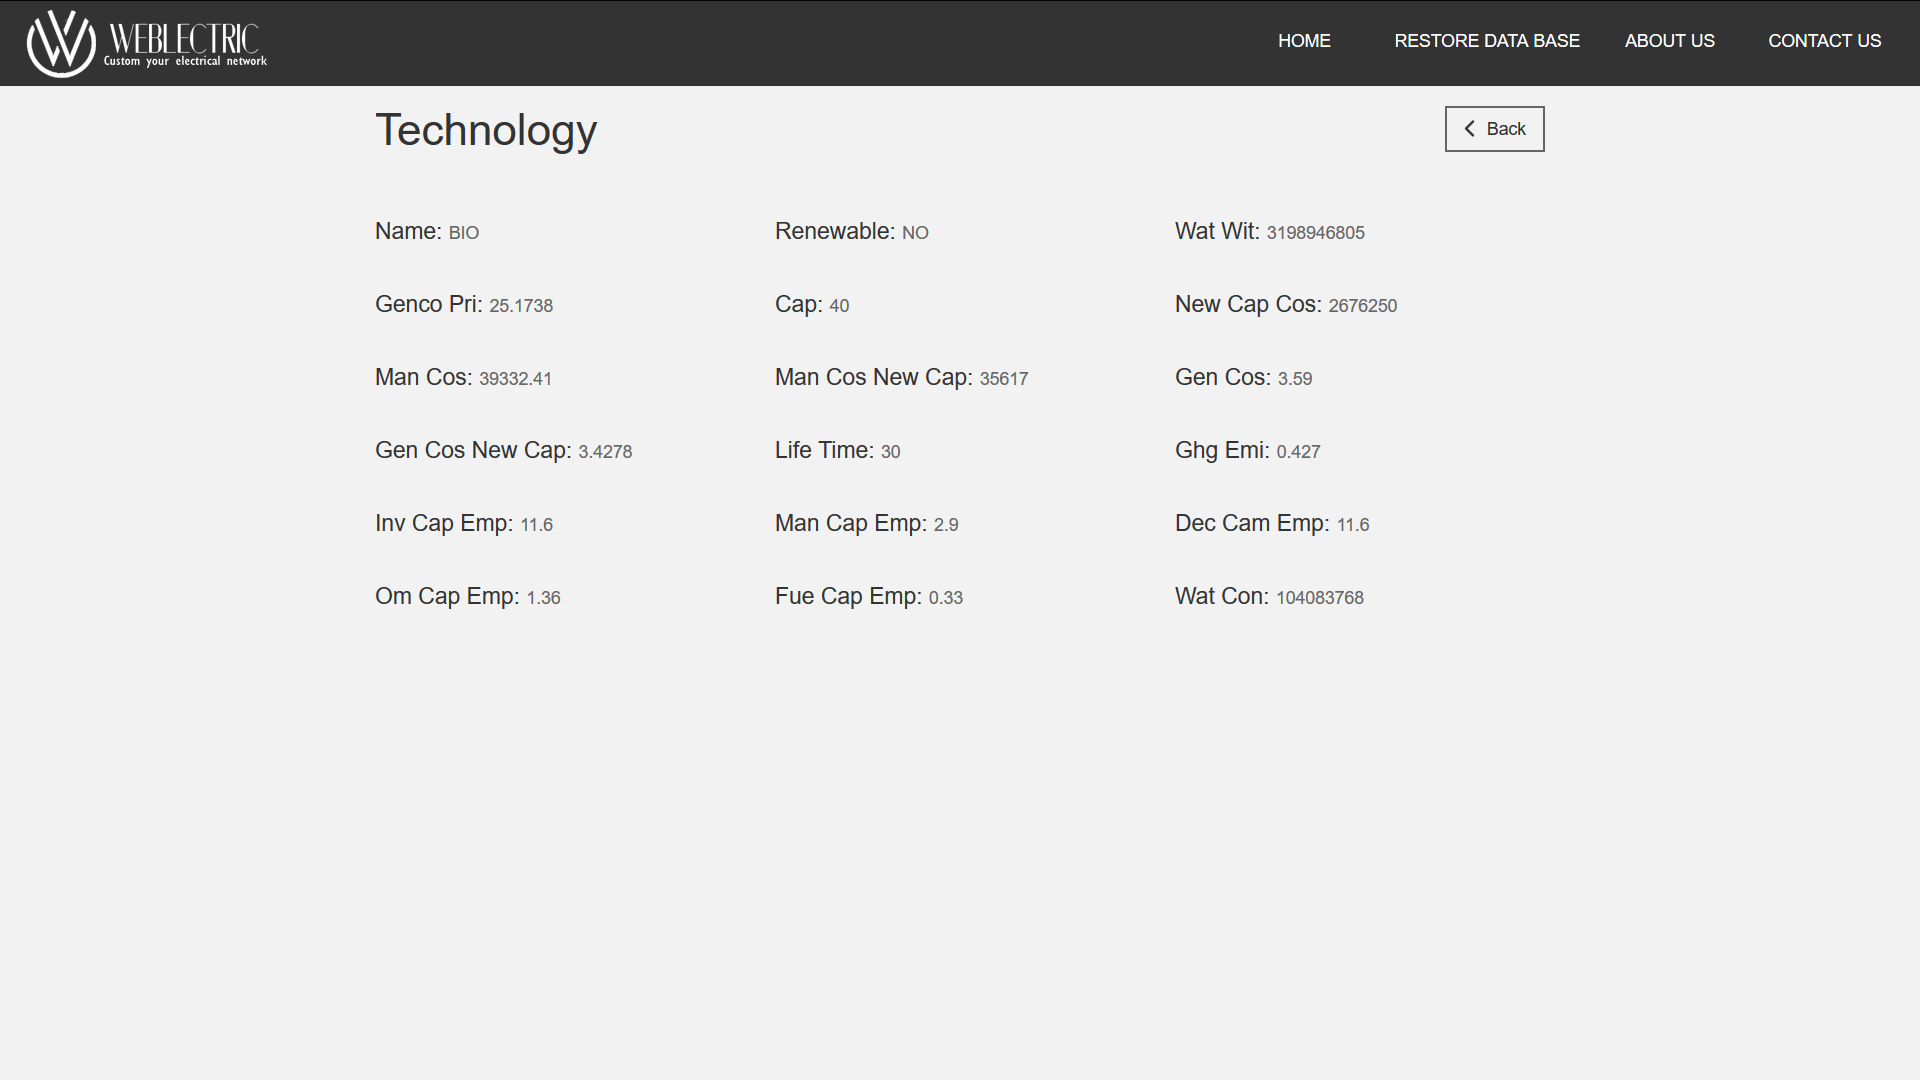
\includegraphics[width=1\textwidth]{/anexos/Diseno/Mockups/FentidadView}
	\caption{Resultado final: Visualización completa de un elemento.}
	\label{img:FentidadView}
\end{figure}

\begin{figure}[h]
	\centering
	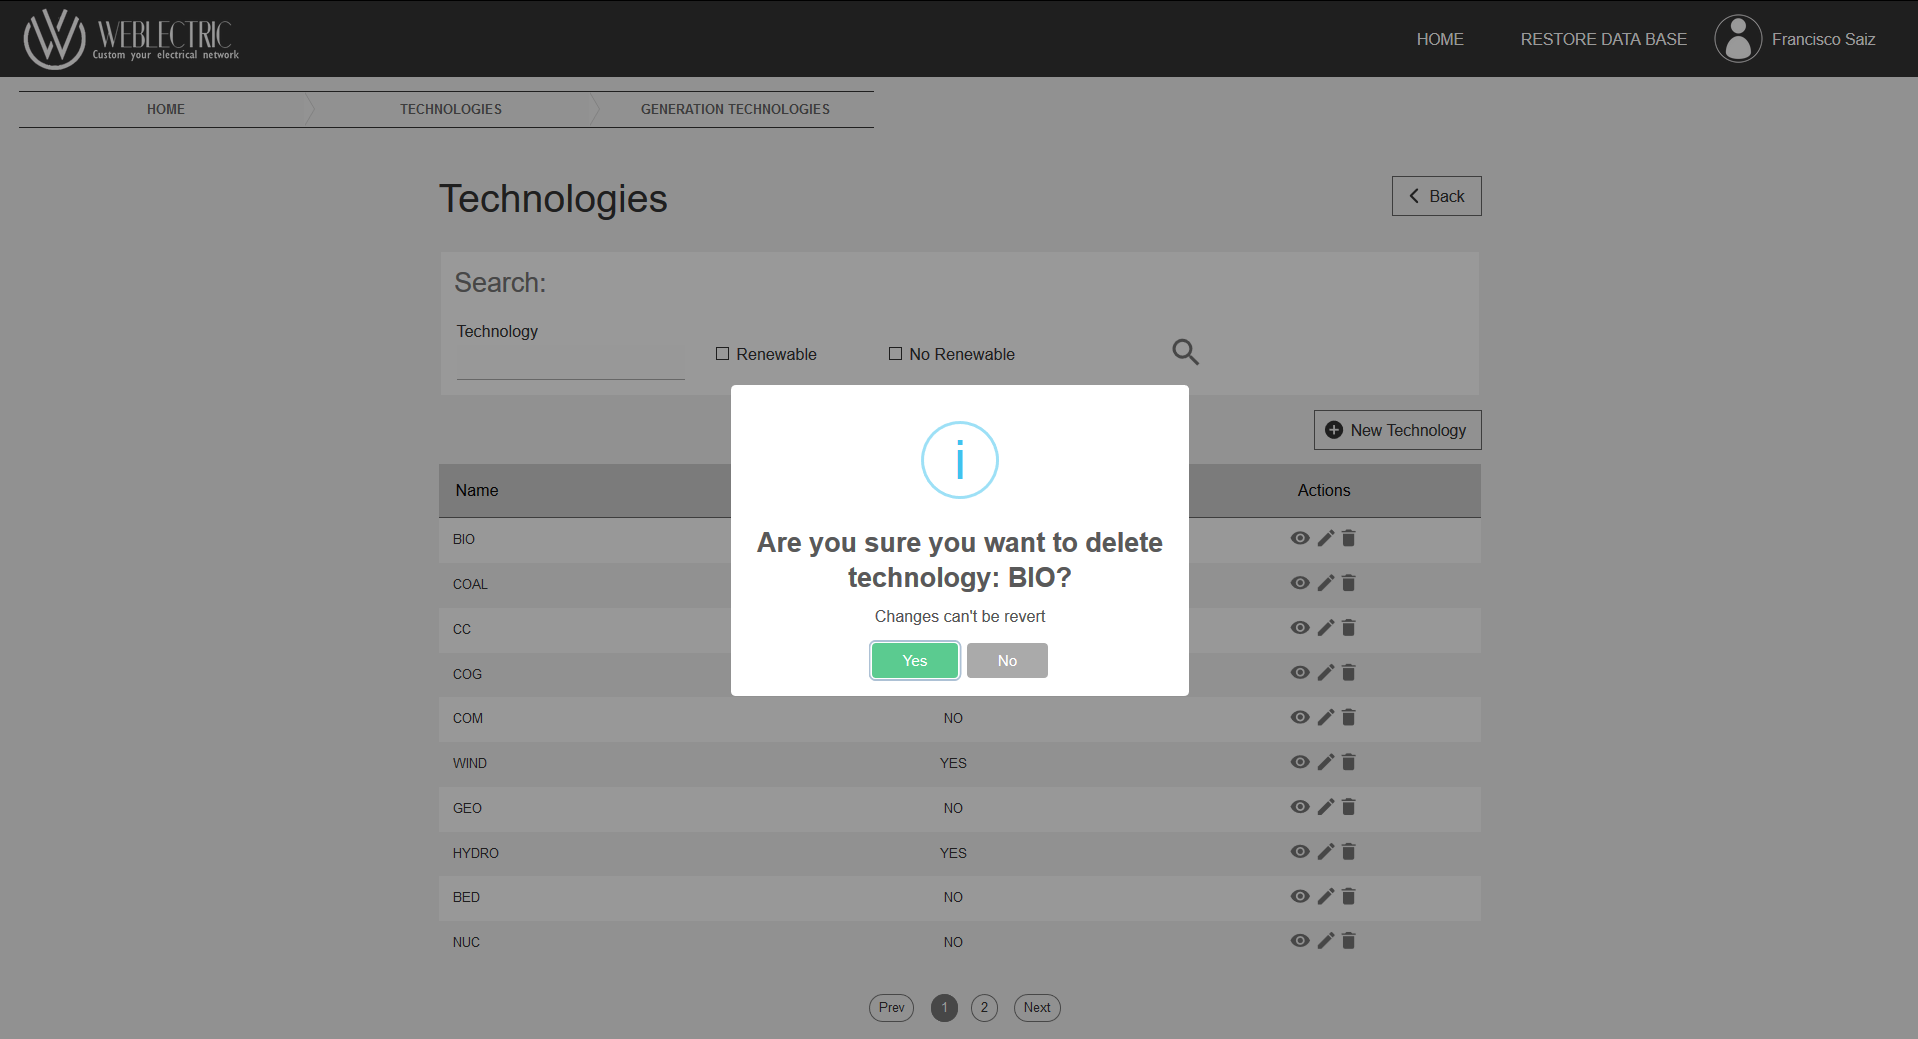
\includegraphics[width=1\textwidth]{/anexos/Diseno/Mockups/FentidadDelete}
	\caption{Resultado final: Mensaje de confirmación al eliminar un elemento.}
	\label{img:FentidadDelete}
\end{figure}

\begin{figure}[h]
	\centering
	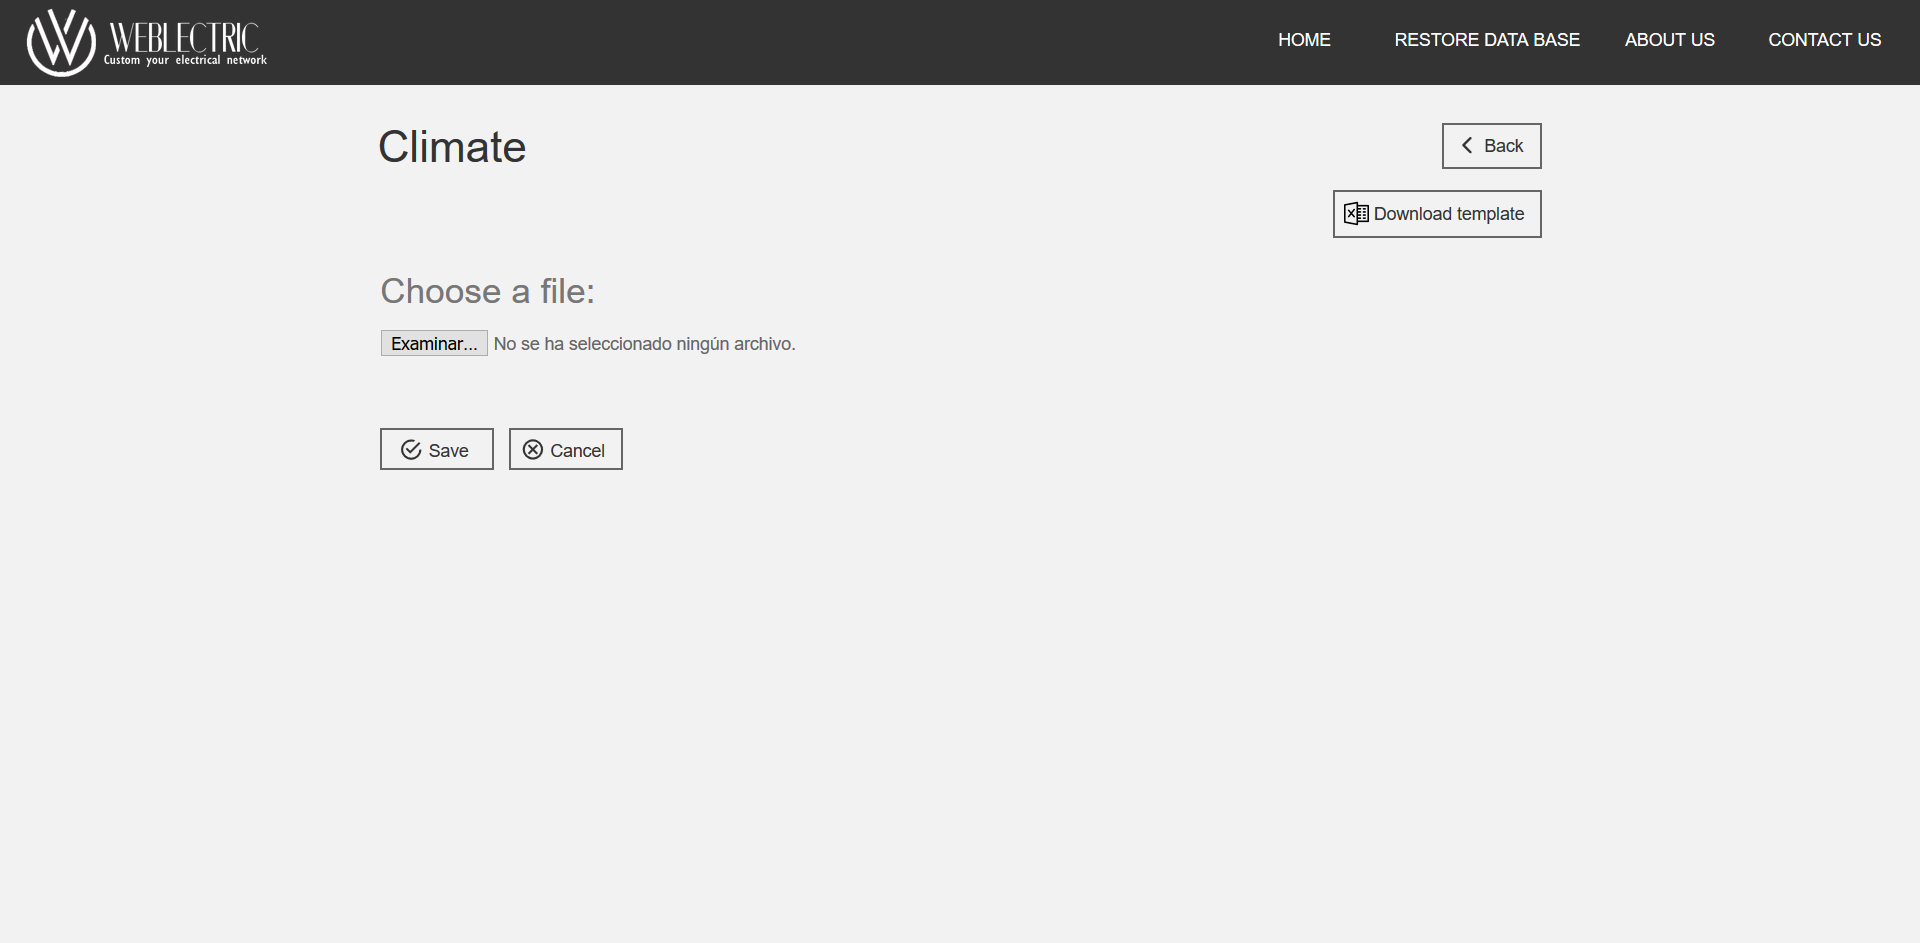
\includegraphics[width=1\textwidth]{/anexos/Diseno/Mockups/FentidadExcel}
	\caption{Resultado final: Administración de entidades mediante hoja de cálculo.}
	\label{img:FentidadExcel}
\end{figure}

\begin{figure}[h]
	\centering
	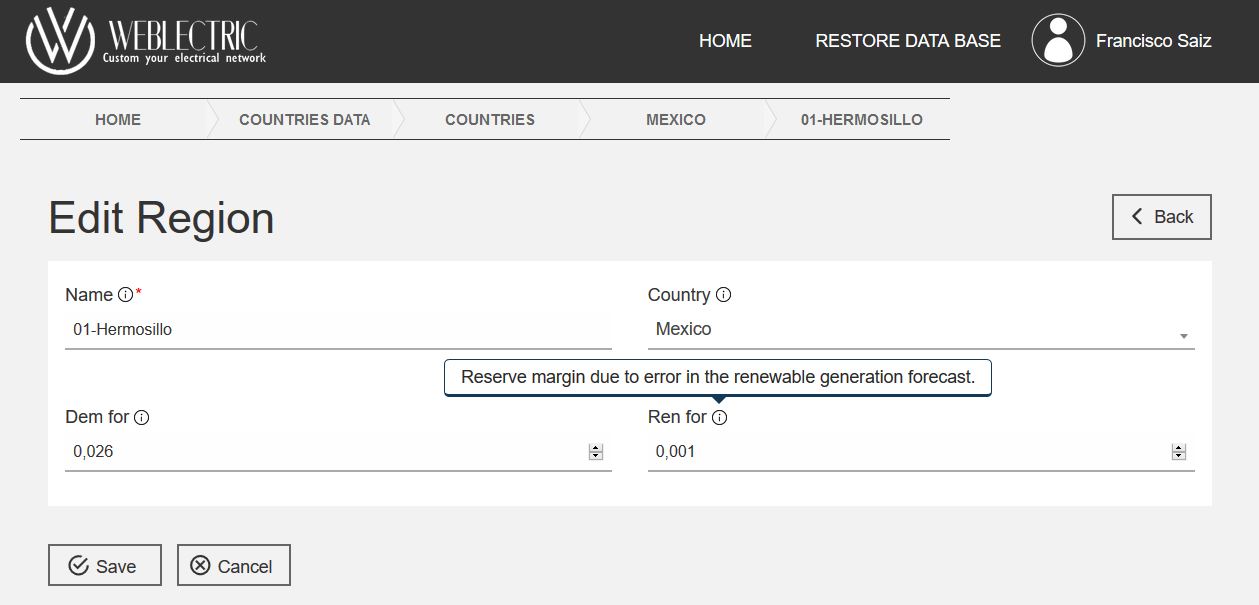
\includegraphics[width=1\textwidth]{/anexos/Diseno/Mockups/Ftooltips}
	\caption{Resultado final: Etiquetas con iconos y títulos, migas de pan y seccion de usuario.}
	\label{img:Ftooltips}
\end{figure}

\begin{figure}[h]
	\centering
	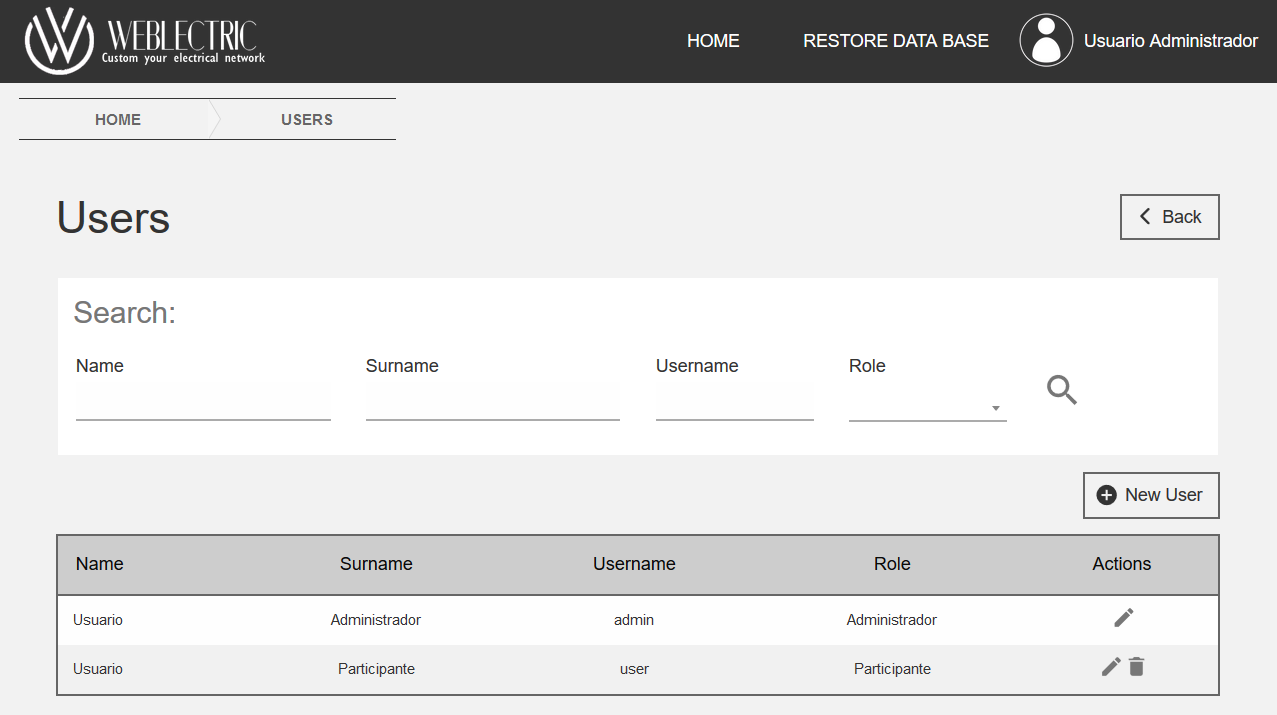
\includegraphics[width=1\textwidth]{/anexos/Diseno/Mockups/Fusers}
	\caption{Resultado final: Pantalla principal de la administración de usuarios.}
	\label{img:Fusers}
\end{figure}

\begin{figure}[h]
	\centering
	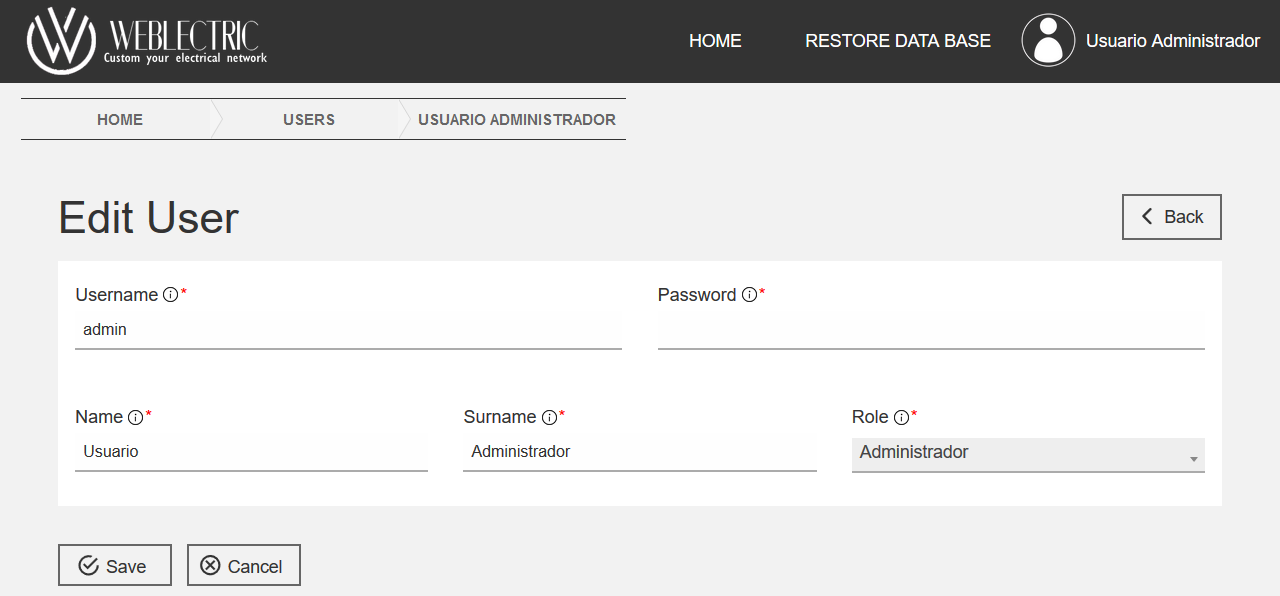
\includegraphics[width=1\textwidth]{/anexos/Diseno/Mockups/Fusersform}
	\caption{Resultado final: Pantalla de edición de un usuario.}
	\label{img:Fusersform}
\end{figure}

\begin{figure}[h]
	\centering
	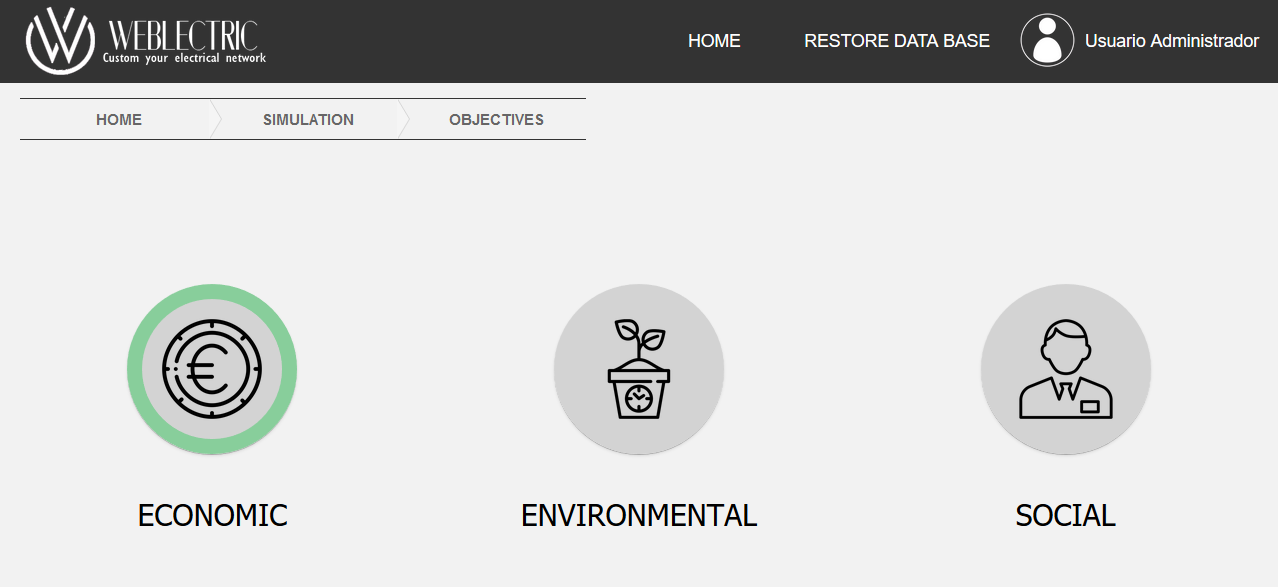
\includegraphics[width=1\textwidth]{/anexos/Diseno/Mockups/Fobjectives}
	\caption{Resultado final: Pantalla donde se representan los tres tipos de objetivos.}
	\label{img:Fobjectives}
\end{figure}

\begin{figure}[h]
	\centering
	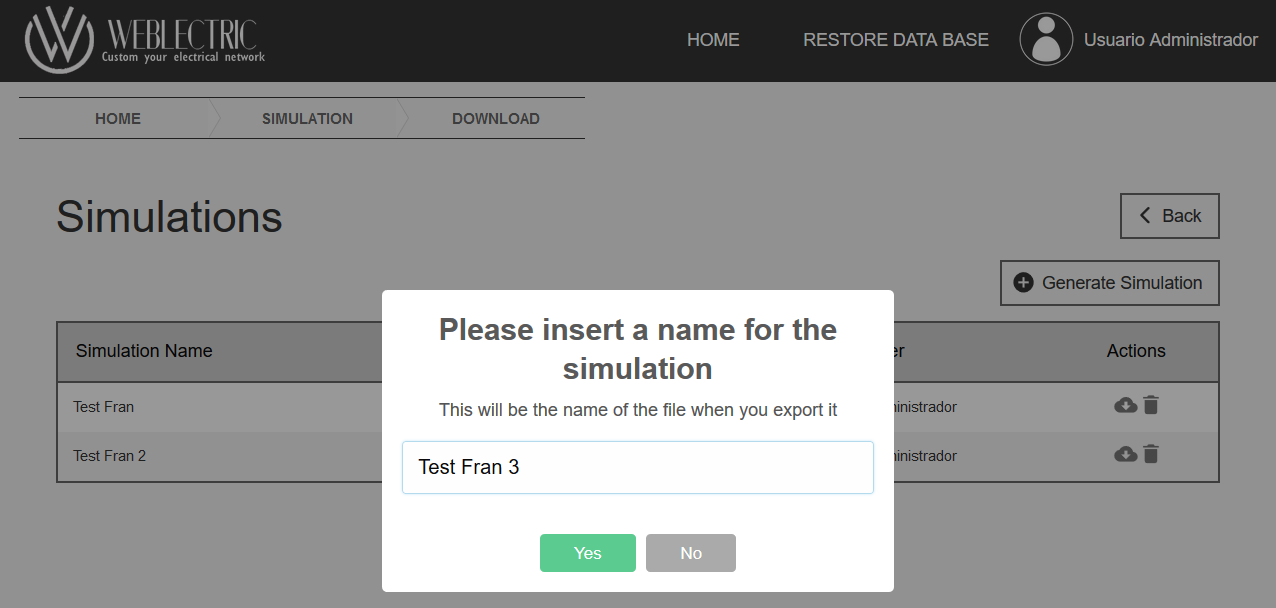
\includegraphics[width=1\textwidth]{/anexos/Diseno/Mockups/Fsimulationname}
	\caption{Resultado final: Ejemplo de creación de una nueva simulación.}
	\label{img:Fsimulationname}
\end{figure}

\begin{figure}[h]
	\centering
	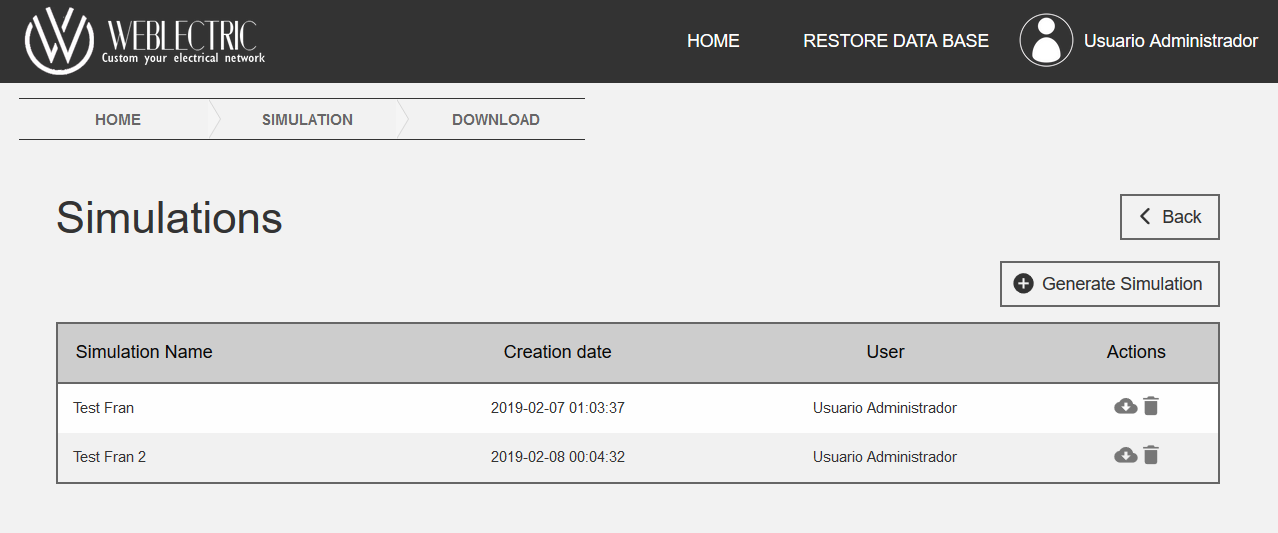
\includegraphics[width=1\textwidth]{/anexos/Diseno/Mockups/Fsimulationdownloads}
	\caption{Resultado final: Pantalla en la que se listan las simulaciones ya creadas y disponibles para descargar.}
	\label{img:Fsimulationdownloads}
\end{figure}